\documentclass[slidestop,aspectratio=169]{beamer}
\usetheme{Pittsburgh}
\usepackage{listings}
\usepackage[utf8x]{inputenc}
\usepackage{etex}
\usepackage[setrelation]{math}
\usepackage[modernsign,substopindex,shortmquant,mquantifiertype,
mconnectiveformal,postfixflatinterpret,bracketmodalinterpret,
setfixinterpret,modifopindex,seqinfers,seqoptional,footnotecalculus,abbrseqcontext,shortterms,nosigmaterms,novarterms]{logic}
\usepackage[pretest,nocommandblocks]{progreg}
\usepackage[bracketinterpret,postfixinterpret,bracketmodalinterpret,simplenames]{dL}
\usepackage{tabularx,xcolor,colortbl}
\usepackage{subcaption}
\usepackage{booktabs}
\usepackage{todonotes}
\usepackage{wrapfig}
\usepackage{stmaryrd}
\usepackage{proof}
\usepackage{prettyref}
\usepackage{tikz}
\usepackage{pgfplots}
\usepackage{slidetool}
\usepackage[absolute,overlay]{textpos}
\usepackage{marvosym}
\let\Cross\undefined
\usepackage{bbding}
\usenavigationsymbolstemplate{}
\pgfplotsset{width=8cm,compat=1.9}
 \usetikzlibrary{arrows}
 \usetikzlibrary{calc}
 \usetikzlibrary{fit}
 \usetikzlibrary{positioning,shadows}
 \usetikzlibrary{automata}
 \usetikzlibrary{shapes,arrows}
 \usetikzlibrary{decorations.text}
 \usetikzlibrary{decorations.markings}
 \usetikzlibrary{trees,snakes}
\usetikzlibrary{pgfplots.dateplot}
\usepackage{relsize}
\tikzset{fontscale/.style = {font=\relsize{#1}}}
\usepackage{pgfplotstable}
\usepackage{filecontents}

\definecolor{vermillion}{rgb}{0.8,0.4,0}
\definecolor{myblue}{rgb}{0,0.45,0.7}
\definecolor{myyellow}{rgb}{0.85,0.8,0.17}


\newcommand{\rref}[2][]{\prettyref{#2}}

  \tikzstyle{noteline}=[shorten <=8pt]%
  \tikzstyle{notebox}+=[minimum height=1.1cm]%
\newrefformat{sec}{Section\,\ref{#1}}
\newrefformat{appendix}{Appendix\,\ref{#1}}
 \newrefformat{model}{Model\,\ref{#1}}
 \newrefformat{listing}{Listing\,\ref{#1}}
 \newrefformat{line}{line\,\ref{#1}}
 \newrefformat{def}{Definition\,\ref{#1}}
 \newrefformat{defn}{Definition\,\ref{#1}}
 \newrefformat{thm}{Theorem\,\ref{#1}}
 \newrefformat{ax}{\ref{#1}}
 \newrefformat{prop}{Proposition\,\ref{#1}}
 \newrefformat{lem}{Lemma\,\ref{#1}}
 \newrefformat{cor}{Corollary\,\ref{#1}}
 \newrefformat{ex}{Example\,\ref{#1}}
 \newrefformat{tab}{Table\,\ref{#1}}
 \newrefformat{fig}{Figure\,\ref{#1}}
 \newrefformat{eqn}{(\ref{#1})}
\renewcommand{\ivr}{\psi}
\providecommand{\tweak}[1]{#1}
\newcommand{\untweak}[1]{}
\newcommand{\ignore}[1]{}
\newcommand{\stdI}{\dLint[state=\nu]}%
\newcommand{\ws}{\nu}
\newcommand{\wt}{\omega}%
\newcommand{\I}{\iconcat[state=\ws]{\stdI}}%
\newcommand{\It}{\iconcat[state=\wt]{\stdI}}%
\definecolor{vgray}{rgb}{.35,.35,.35}
\renewcommand*{\irrulename}[1]{\text{\textcolor{vgray}{\upshape#1}}}
\usepackage{tikz}
\usepackage{stmaryrd}
\usetikzlibrary{arrows,matrix}
\newcommand{\isabelle}{Isabelle/HOL\xspace}
\newcommand{\allstate}{\mathcal{S}}
\newcommand{\tvm}{\oslash}
\newcommand{\tvt}{\oplus}
\newcommand{\tvf}{\ominus}
\newcommand{\term}{\mathbf{Term}\xspace}
\newcommand{\lequiv}{\leftrightarrow}
\newcommand{\state}{\mathbf{State}\xspace}
\newcommand{\prop}{\mathbf{Prop}\xspace}
\newcommand{\fml}{\mathbf{Fml}\xspace}
\newcommand{\dLi}{\ensuremath{\dL_{\iota}}\xspace}
\newcommand{\KeY}{KeY}
\newcommand{\tint}[2]{#2\lenvelope#1\renvelope}
\newcommand{\fint}[2]{#2\lenvelope#1\renvelope}
\newcommand{\pint}[1]{\lenvelope#1\renvelope}
\newcommand{\piint}[2]{#2\lenvelope#1\renvelope}
\newcommand{\meps}[2]{\iota{#1}\,{#2}}
\newcommand{\mepsIndef}[2]{\varepsilon{#1}\,{#2}}
\newcommand{\R}{\mathbb{R}}
\newcommand{\err}{\textsf{Err}\xspace}
\newcommand{\ffalse}{\textsf{false}\xspace}
\newcommand{\ftrue}{\textsf{true}\xspace}
\newcommand{\projGen}[2]{\ensuremath{\pi_{#1}}{#2}}
\newcommand{\projL}[1]{\projGen{1}{#1}}
\newcommand{\projR}[1]{\projGen{2}{#1}}
\newcommand{\inR}[1]{\textsf{in}{\ensuremath{\mathbb{R}}}(#1)}
\newcommand{\isT}[1]{\textsf{isT}(#1)}
\newcommand{\om}{\omega}
\newcommand{\tom}{\tilde{\omega}}
\newcommand{\tnu}{\tilde{\nu}}
\newcommand{\tmu}{\tilde{\mu}}
\newcommand{\denote}[1]{\mathsf{E}(#1)}
\newcommand{\llc}[3]{\mathsf{LLC}(#2(#1))}
\newcommand{\cont}[2]{\mathsf{Con}(#2(#1))}
\newcommand{\tder}[2]{\der{#2(#1)}}
\newcommand{\hasdiff}[1]{\mathsf{D}(#1)}
\newcommand{\vepsilon}{\xi}
\newcommand{\stepsto}{\allowbreak\mapsto\allowbreak}
\newcommand{\bebecomes}{\mathrel{::=}}
\newcommand{\alternative}{~|~}
\newcommand{\ProofPlex}{ProofPlex\xspace}
\newcommand{\ModelPlex}{ModelPlex\xspace}
\providecommand{\KeYmaeraX}{KeYmaera X\xspace}


% CdGL
\newcommand{\GL}{GL\xspace}
\newcommand{\CGL}{CGL\xspace}
\newcommand{\CdGL}{CdGL\xspace}
\newcommand{\dRL}{dRL\xspace}
\newcommand{\Isabelle}{Isabelle\xspace}
\newcommand{\CakeML}{CakeML\xspace}
\newcommand{\rangevar}{\textsf{Range}}
\newcommand{\testvar}{\textsf{test}}
\newcommand{\elem}[2]{\textsf{Dec}[#1](#2)}
\newcommand{\spc}{\hspace{0.15in}}
\newcommand{\kwmod}{\textsf{mod}}
\newcommand{\emod}[2]{#1~\kwmod~#2}
\newcommand{\kwdiv}{\textsf{div}}
\newcommand{\ediv}[2]{#1~\kwdiv~#2}
\newcommand{\kwsig}{\Sigma}
\newcommand{\sig}[1]{\kwsig(#1)}
\newcommand{\interp}{I}
\newcommand{\valset}[1]{\mathfrak{V}(#1)}
\newcommand{\kwbool}{\m{\mathbb{B}}}
\newcommand{\kwint}{\m{\mathbb{Z}}}
\newcommand{\kwreal}{\m{\mathbb{R}}}
\newcommand{\kwintsig}{\Xi}
\newcommand{\intsig}[1]{\kwintsig(#1)}
\newcommand{\churchkleene}{\omega_{\text{CK}}}
\newcommand{\restL}[1]{#1_L}
\newcommand{\restR}[1]{#1_R}
\newcommand{\apL}[1]{#1_{\langle{0}\rangle}}
\newcommand{\apR}[1]{#1_{\langle{1}\rangle}}
\newcommand{\dpL}[1]{#1_{[0]}}
\newcommand{\dpR}[1]{#1_{[1]}}
\newcommand{\va}{a}
\newcommand{\vb}{b}
\newcommand{\vca}{\overline{a}}
\newcommand{\vcb}{\overline{b}}
\newcommand{\btt}{\texttt{tt}}
\newcommand{\bff}{\texttt{ff}}
\newcommand{\stt}{\textsf{early\_win}}
\newcommand{\sff}{\textsf{early\_loss}}
\newcommand{\demonactive}[2]{\textrm{aD}(#1,#2)}
\newcommand{\demondormant}[2]{\textrm{dD}(#1,#2)}
\newcommand{\sren}[3]{\urename[{#1}]{#2}{#3}}%{\subst[{#1}]{#2}{#3}}
\newcommand{\ssub}[3]{\subst[{#1}]{#2}{#3}}
\newcommand{\eren}[3]{\urename[{#1}]{#2}{#3}}%{\subst[{#1}]{#2}{#3}}
\newcommand{\earen}[2]{\urename[{#1}]{\boundvars{#2}}{\vec{y}}}%{\subst[{#1}]{\boundvars{#2}}{\vec{y}}}
\newcommand{\allcon}{\allregion}
\newcommand{\somesemi}[2]{\epsilon #1~|~#2}
\newcommand{\rzF}[2]{#1 \vdash #2}
\newcommand{\rzA}[3]{\langle{#2}\rangle(#1)=(#3)}
\newcommand{\rzD}[3]{[{#2}](#1)=(#3)}
\newcommand{\rzFst}[1]{#1_0}
\newcommand{\rzSnd}[1]{#1_1}
\newcommand{\rzThd}[1]{#1_2}
\newcommand{\rzFrt}[1]{#1_3}
\newcommand{\rzApp}[2]{#1\,#2}
\newcommand{\sa}{\omega}
\renewcommand{\sb}{\nu}
\newcommand{\Sc}{\mu}
\renewcommand{\aa}{a}
\newcommand{\ab}{b}
\newcommand{\ac}{c}
\newcommand{\da}{d}
\newcommand{\db}{D}
\newcommand{\dc}{\DJ}
\newcommand{\allRz}{\mathcal{R}\mathbf{z}}
\newcommand{\rzfor}[1]{#1\,\allRz}
\newcommand{\mto}{\rightharpoonup}
\newcommand{\esub}[3]{[{#3}/{#2}]{#1}}
\newcommand{\tsub}[3]{\subst[#1]{#2}{#3}}
%\newcommand{\rzF}[2]{#1 \vdash #2}
%\newcommand{\rzA}[3]{\langle{#2}\rangle(#1)=(#3)}
%\newcommand{\rzD}[3]{[{#2}](#1)=(#3)}
\newcommand{\rzNil}{\epsilon}
\newcommand{\rzCons}[2]{(#1,#2)}
\newcommand{\rzBLam}[2]{\lambda #1:\allstate.~#2}
\newcommand{\rzHOLam}[3]{\Lambda #1:\rzfor{#2}.~#3}
\newcommand{\rzFOLam}[3]{\Lambda #1:#2.~#3}
%\newcommand{\rzApp}[2]{#1\,#2}
\newcommand{\fintR}[1]{\fint{#1}{}} %{#1#2}
\newcommand*{\strategyforR}[2][]{{#2}\Langle{#1}\Rangle}
\newcommand*{\istrat}[3][]{\strategyforR[#1]{#2}^{#3}}
\newcommand*{\dstrategyforR}[2][]{{#2}\lenvelopewide{#1}\renvelopewide}
%{{#2}\llbracket{#1}\rrbracket}
\newcommand*{\idstrat}[3][]{\dstrategyforR[#1]{#2}^{#3}}
\newcommand{\cint}[1]{\fint{\bigwedge #1}}
\newcommand{\cintR}[1]{\fintR{\bigwedge #1}}
\newcommand{\seq}[2]{#1 \vdash #2}
\newcommand{\proves}[3]{#1\allowbreak\vdash #2 \allowbreak \mathop{:} #3}
\newcommand{\edOpencons}{\langle}
\newcommand{\edClosecons}{\rangle}
\newcommand{\edSepcons}{,}
\newcommand{\edcons}[2]{\edOpencons{#1}\edSepcons{#2}\edClosecons}
%\newcommand{\edcons}[2]{\langle#1,#2\rangle}
\newcommand{\ebOpencons}{[}
\newcommand{\ebSepcons}{,}
\newcommand{\ebClosecons}{]}
\newcommand{\ebcons}[2]{\ebOpencons#1\ebSepcons#2\ebClosecons}
\newcommand{\eCons}[2]{\lstrike{#1,#2}\rstrike}
\newcommand{\eSnoc}[2]{\llensehat{#1,#2}\rlensehat}
\newcommand{\pmodality}[2]{\llensehat{#1}\rlensehat{#2}}
\newcommand{\econs}[2]{\eCons{#1}{#2}}
\newcommand{\einjL}[1]{\ell \cdot #1}
\newcommand{\einjR}[1]{r \cdot #1}
\newcommand{\kwcase}{\textrm{case}}
\newcommand{\ecaseHead}[1]{\langle\kwcase\textrm{ }#1{\text{\textrm{ of }}}}
\newcommand{\ecaseLeft}[2]{#1\Rightarrow~#2}
\newcommand{\ecaseRight}[2]{~|~#1\Rightarrow~#2}
\newcommand{\ecaseEnd}{\rangle}
\newcommand{\ecasegen}[5]{\ecaseHead{#1}\allowbreak\ecaseLeft{#2}{#3}\allowbreak\ecaseRight{#4}{#5}\ecaseEnd}
\newcommand{\ecase}[3]{\ecasegen{#1}{\ell}{#2}{r}{#3}}
\newcommand{\edcase}[3]{\ecase{#1}{#2}{#3}}
\newcommand{\ercase}[3]{\langle\textrm{case}_*\ #1\text{ of }\pvs\Rightarrow~#2~|~\pvg\Rightarrow#3\rangle}
\newcommand{\eCase}[3]{\lstrike\kwcase\textrm{ }#1\textrm{ of }\allowbreak\ell\Rightarrow~#2~\allowbreak|~r\Rightarrow~#3\rstrike} %\{\textrm{case}\}\ #1\textrm{ of }\ell.~#2~|~r.~#3
\newcommand{\edinjL}[1]{\langle\ell \cdot #1\rangle}
\newcommand{\edinjR}[1]{\langle r \cdot #1\rangle}
\newcommand{\eInjL}[1]{\lstrike\ell \cdot #1\rstrike}
\newcommand{\eInjR}[1]{\lstrike{r \cdot #1}\rstrike}
\newcommand{\kwrep}{\textrm{rep}}
\newcommand{\erep}[3]{{#1}\textrm{ }\kwrep\text{ }#3.~{#2}}
\newcommand{\eapp}[2]{#1\ #2}
\newcommand{\elamgen}[3]{\lambda #1:#2.~ #3}
\newcommand{\eplam}[2]{\elamgen{\pvx}{#1}{#2}}
\newcommand{\etlam}[2]{\elamgen{x}{#1}{#2}}
\newcommand{\ebseq}[1]{[\iota~#1]}
\newcommand{\ebseqinv}[1]{[\iota~{#1}^{-1}]}
\newcommand{\edseq}[1]{\langle\iota~#1\rangle}
\newcommand{\edseqinv}[1]{\langle\iota~{#1}^{-1}\rangle}
\newcommand{\eSeq}[1]{\lstrike\iota~#1\rstrike}
\newcommand{\eSeqinv}[1]{\lstrike\iota~{#1}^{-1}\rstrike}
\newcommand{\ebOpenswap}{[\textrm{yield }}
\newcommand{\ebCloseswap}{]}
\newcommand{\ebswap}[1]{\ebOpenswap#1\ebCloseswap}
\newcommand{\edOpenswap}{\langle\textrm{yield }}
\newcommand{\edCloseswap}{\rangle}
\newcommand{\edswap}[1]{\edOpenswap#1\edCloseswap}
%\llensehat \rlensehat  \lstrike \rstrike
\newcommand{\eSwap}[1]{\lstrike\textrm{yield }#1\rstrike}
\newcommand{\ePaws}[1]{\llensehat\textrm{yield }#1\rlensehat}
\newcommand{\emonInfix}[1]{{\circ_{#1}}}
\newcommand{\emon}[3]{{#1} \emonInfix{#3} {#2}}
%\newcommand{\eQEpos}{\textrm{QE}_{pos}}
%\newcommand{\eQEneg}{\textrm{QE}_{neg}}
\newcommand{\eQE}[2]{\textsf{FO}[#1](#2)}
%\newcommand{\eQEN}[1]{\textsf{QE}[#1]_\mathbb{N}}
%\newcommand{\eQER}[1]{\textsf{QE}[#1]_\mathbb{R}}
\newcommand{\emetsplit}{\textrm{split}\met}
\newcommand{\esplit}[3]{\textrm{split }{[#1\sim#2]}~#3}
\newcommand{\kwstop}{\textrm{stop}}
\newcommand{\kwgo}{\textrm{go}}
\newcommand{\estop}[1]{\langle\kwstop\ #1\rangle}
\newcommand{\ego}[1]{\langle\kwgo\ #1\rangle}
\newcommand{\kwroll}{\textrm{roll}}
\newcommand{\kwunroll}{\textrm{unroll}}
\newcommand{\ebroll}[1]{[\kwroll\ {#1}]}
\newcommand{\ebunroll}[1]{[\kwunroll\ #1]}
\newcommand{\eRoll}[1]{\lstrike\kwroll\ #1\rstrike}
\newcommand{\eUnroll}[1]{\lstrike\kwunroll\ #1\rstrike}
\newcommand{\eghost}[4]{\textrm{Ghost}[#1=#2](#3.~#4)}
\newcommand{\eAsgn}[4]{\lstrike\humod{#2}{\eren{f}{#2}{#1}}\text{ in }#3.~#4\rstrike}
\newcommand{\eAsgneq}[4]{\eAsgn{#1}{#2}{#3}{#4}}
\newcommand{\etconsgen}[5]{\langle{\eren{#4}{#1}{#2}}~{{:}{*}}~#3.~#5\rangle}
\newcommand{\etcons}[2]{\etconsgen{x}{y}{\pvx}{#1}{#2}}
\newcommand{\ietcons}[3]{\langle{\eren{#2}{#1}{~}}~{{:}{*}}~#3\rangle}
\newcommand{\ebasgneq}[4]{[\humod{#2}{\eren{f}{#2}{#1}}\text{ in }#3.~#4]}
\newcommand{\edasgneq}[4]{\langle\humod{#2}{\eren{f}{#2}{#1}}\text{ in }#3.~#4\rangle}
\newcommand{\edasgn}[4]{\edasgneq{#1}{#2}{#3}{#4}}
\newcommand{\ebasgn}[4]{\ebasgneq{#1}{#2}{#3}{#4}}
\newcommand{\iebasgn}[2]{[\humod{#1}{\eren{f}{#1}{~}}\text{ in }~#2]}
\newcommand{\iedasgn}[2]{\langle\humod{#1}{\eren{f}{#1}{~}}\text{ in }~#2\rangle}
%\newcommand{\iedasgn}[2]{\edasgneq{~}{#1}{#1}{#2}}
%\newcommand{\iebasgn}[2]{\ebasgneq{~}{#1}{#1}{#2}}
\newcommand{\eunpack}[2]{\textrm{unpack}(#1,\pvx y.~#2)}
\newcommand{\ewhile}[2]{\textrm{while}(#1 > 0)\{#2\}}
\newcommand{\eloopelim}[3]{(#1, x.~{#2}^{#3})}
\newcommand{\efpgen}[5]{\textit{FP}(#1, #2.~#3, #4.~#5)}
\newcommand{\efp}[3]{\efpgen{#1}{\pvs}{#2}{\pvg}{#3}}
\newcommand{\met}{\ensuremath{\mathcal{M}}}
\newcommand{\conv}{\varphi\xspace}
\newcommand{\G}{\Gamma}
\newcommand{\Gemp}{\cdot}
\newcommand{\issimp}[1]{{#1}\ \textrm{simp}}
\newcommand{\eforHead}[4]{\textrm{for}(#1:\conv(\met)={#2};#3;{#4})} %#3:\met>0\land\met_0=\met
\newcommand{\eforBody}[1]{\{#1\}}
\newcommand{\eforgen}[5]{\eforHead{#1}{#2}{#3}{#4}\eforBody{#5}}
\newcommand{\efor}[2]{\eforgen{\pvx}{#1}{\pvy}{#2}{\alpha}}
\newcommand{\oldof}[1]{\textrm{old}(#1)}
\newcommand{\isnorm}[1]{#1\text{ normal}}
\newcommand{\pvx}{p}
\newcommand{\pvy}{q}
\newcommand{\pvz}{t}
\newcommand{\pvl}{\ell}
\newcommand{\pvr}{r}
\newcommand{\pvrr}{rr}
\newcommand{\pvs}{s}
\newcommand{\pvg}{g}
\newcommand{\sdual}[1]{\pdual{#1}}



%%% KAISAR
\newcommand{\spost}[2]{\mathsf{sp}(#1,#2)}
\newcommand{\kwassume}{\textbf{assume}}
\newcommand{\kwassert}{\textbf{assert}}
\newcommand{\kwlet}{\textbf{let}}
\newcommand{\kwstate}{\textbf{state}}
\newcommand{\kwsolve}{\textbf{solve}}
\newcommand{\kwshow}{\textbf{show}}
%\newcommand{\kwassume}{\textbf{assume}}
\newcommand{\kwby}{\textbf{by}}
\newcommand{\kwusing}{\textbf{using}}
\newcommand{\kwnote}{\textbf{note}}
\newcommand{\kwhave}{\textbf{have}}
\newcommand{\kwinv}{\textbf{inv}}
\newcommand{\kwghost}{\textbf{Ghost}}
\newcommand{\kwind}{\textbf{Ind}}
\newcommand{\kwpre}{\textbf{Pre}}
\newcommand{\kwfinally}{\textbf{finally}}
\newcommand{\kwassign}{\textbf{assign}}
\newcommand{\kwmid}{\textbf{after}}
\newcommand{\kwfirst}{\textbf{have}}
\newcommand{\kwthen}{\textbf{then}}
%\newcommand{\kwcase}{\textbf{case}}
\newcommand{\kwfocus}{\textbf{focus}}
\newcommand{\semiset}[2]{\{#1~|~#2\}} 
\newcommand{\sshow}[3]{\textsf{show}~{#1}:{#2}~{#3}}
\newcommand{\shave}[4]{\textsf{have}~{#1}:{#2}~{#3}~{#4}}
\newcommand{\snote}[4]{\textsf{note}~{#1}:{#2}~{#3}~{#4}}


% END-TO-END
\newcommand{\xgivar}{\textsf{xi}}
\newcommand{\ygivar}{\textsf{yi}}
\newcommand{\xgvar}{\textsf{x}}
\newcommand{\ygvar}{\textsf{y}}
\newcommand{\xcvar}{\textsf{xc}}
\newcommand{\ycvar}{\textsf{yc}}
\newcommand{\ytvar}{\textsf{yt}}
%\newcommand{\xivar}{\textsf{xi}}
%\newcommand{\yivar}{\textsf{yi}}
%\newcommand{\xvar}{\textsf{x}}
\newcommand{\yvar}{\textsf{y}}
\newcommand{\wvar}{\textsf{w}}
\newcommand{\dxvar}{\textsf{dx}}
\newcommand{\dyvar}{\textsf{dy}}
\newcommand{\dxivar}{\textsf{dxi}}
\newcommand{\dyivar}{\textsf{dyi}}
\newcommand{\dxgvar}{\textsf{dxg}}
\newcommand{\dygvar}{\textsf{dyg}}
\newcommand{\kvar}{\textsf{k}}
\newcommand{\tvar}{\textsf{t}}
\newcommand{\vivar}{\textsf{vi}}
\newcommand{\vlvar}{\textsf{vl}}
\newcommand{\vhvar}{\textsf{vh}}
\newcommand{\obsvar}{{\sf obs}\xspace}
\newcommand{\Tvar}{{\sf T}\xspace}
\newcommand{\Avar}{{\sf A}\xspace}
\newcommand{\Bvar}{{\sf B}\xspace}
%\newcommand{\SBvar}{{\it SB }\xspace}
\newcommand{\xvar}{{\sf x}\xspace}
\newcommand{\vvar}{{\sf v}\xspace}
\newcommand{\avar}{{\sf a}\xspace}
\newcommand{\ctrl}{\textsf{ctrl}\xspace}
\newcommand{\ctrlliv}{\ctrl_{\text{a}}}
\newcommand{\plant}{\textsf{plant}\xspace}
\newcommand{\psimp}{\ensuremath{\alpha_{SV}}\xspace}
\newcommand{\sandbox}{\textsf{\upshape sandbox}\xspace}
\newcommand{\fallback}{\textsf{\upshape fallback}\xspace}
\newcommand{\ctrlMon}{\textsf{\upshape ctrlMon}\xspace}
\newcommand{\plantMon}{\textsf{\upshape plantMon}\xspace}
\newcommand{\extCtrl}{\textsf{\upshape extCtrl}\xspace}
\newcommand{\verifiedmodelbody}{\ensuremath{\ctrl;\plant}}
\newcommand{\verifiedmodel}{\ensuremath{\prepeat{(\verifiedmodelbody)}}}
\newcommand{\exctrl}{\textsf{ctrl}_{SV}\xspace}
\newcommand{\pdrive}{\textsf{go}\xspace}
\newcommand{\pstop}{\textsf{stop}\xspace}
\newcommand{\explant}{\textsf{plant}_{SV}\xspace}
\newcommand{\lnorm}[1]{{{\norm{#1}}_{\infty}}}
\newcommand{\enorm}[1]{\norm{#1}}
\newcommand{\linv}{J}
\newcommand{\goback}{\!\!\!\!}
\newcommand{\textbt}[1]{{\text{\ttfamily\fontseries{b}\selectfont #1}}}
\newcommand{\short}{\\[-0.03in]}
\newcommand{\extern}{myyellow}



%Presentation

\theoremstyle{plain}
\theoremstyle{definition}
\theoremstyle{remark}
\definecolor{vermillion}{rgb}{0.8,0.4,0}
\definecolor{myblue}{rgb}{0,0.45,0.7}
\definecolor{myyellow}{rgb}{0.7,0.4,0.10}
\definecolor{semblue}{rgb}{0,0,0.7}
\definecolor{vgreen}{rgb}{.1,.5,0}
\definecolor{vdarkgreen}{rgb}{.06,.3,0}
\definecolor{vred}{rgb}{.7,0,0}
\definecolor{vblue}{rgb}{.1,.15,.62}
\definecolor{vgray}{rgb}{.35,.35,.35}
\definecolor{darkishgray}{rgb}{.35,.35,.35}
\definecolor{vvblue}{rgb}{.14,.21,.868}%{1.4*vblue}
\definecolor{lsblue}{HTML}{16303A}
\definecolor{lslightblue}{HTML}{2E6579}
\definecolor{lsverylightblue}{HTML}{4699B9}
\definecolor{lsgreen}{HTML}{5ECEF9}
\definecolor{lslightgreen}{HTML}{54B9DF}
\definecolor{lsred}{HTML}{B94D5D}
\definecolor{lslightred}{HTML}{F16579}
\definecolor{lsdarkred}{HTML}{3A181D}
\definecolor{smigreen}{RGB}{61,113,120}
\definecolor{smiwhite}{RGB}{221,221,221}
\definecolor{smiblack}{RGB}{25,25,25}
\definecolor{smidarkgray}{RGB}{50,50,50}
\definecolor{smigray}{RGB}{90,90,90}
\definecolor{smired}{RGB}{127,0,0}

\newcommand{\engineer}[1][1in]{
\includegraphics[width=#1]{img/rosie.png}}
\newcommand{\logician}[1][1in]{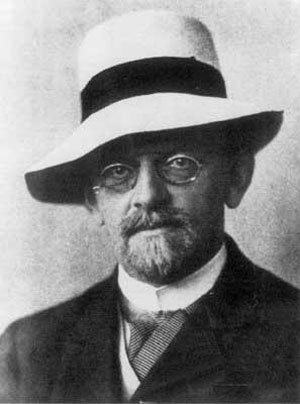
\includegraphics[width=#1]{img/hilbert.png}}
\newcommand{\logicuser}[1][1in]{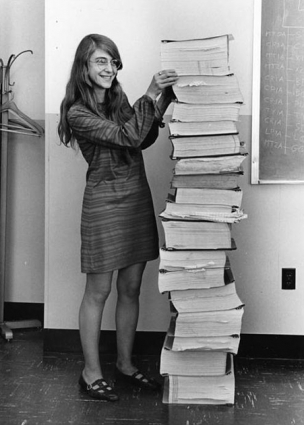
\includegraphics[width=#1]{img/hamilton.png}}
\newcommand{\speak}[2]{\small\begin{minipage}{1.3in}{#1}{#2}\end{minipage}}
\newcommand{\say}[1]{\speak{#1}{}}
%TODO: Color the smiley and frowny for readability
\newcommand{\sayHappy}[1]{\speak{#1}{\color{vgreen}{\Smiley}}}
\newcommand{\saySad}[1]{\speak{#1}{\color{vred}{\Frowny}}}
\newcommand{\turn}{\textsc{Turn}}
\newcommand{\nim}{\textsc{Nim}}
\newcommand{\cake}{\textsc{CC}}
\newcommand{\ah}[2]{\action<#1-|alert@#1>{#2}}
\newcommand{\acl}[2]{\action<#1->{#2}}

\newcommand{\ctrlcolor}[1]{{\color{vred}{#1}}}
\newcommand{\plantcolor}[1]{{\color{vblue}{#1}}}

\title{Practical, End-to-End Verification for Cyber-Physical Systems}
\author{Brandon Bohrer}
\institute[Thesis Committee] % (optional, but mostly needed)
{
  Andr\'{e} Platzer\\
  Stefan Mitsch\\
  Frank Pfenning\\
  Bradley Schmerl, ISR\\
  Tobias Nipkow, TU Munich
}
\date{Thesis Proposal\\October 25 2019}
\setbeamertemplate{footline}[frame number]
\AtBeginSection[]{
  \begin{frame}<beamer>{Outline}
    \tableofcontents[currentsection]
  \end{frame}
}
\AtBeginSubsection[]
{
  \begin{frame}<beamer>{Outline}
    \tableofcontents[currentsection,currentsubsection] 
 \end{frame}
}

\begin{document}
\begin{frame}
  \titlepage
\end{frame}

\section{Introduction}
%%%  If I bring this slide back, connect pictures to next slide
%\begin{frame}[t]{\only<1>{Safety-Critical CPS Need Safety}
%\only<2->{Safety-Critical CPS Need Proofs}}
%  \begin{center}
%    \begin{tabular}{ccc}
%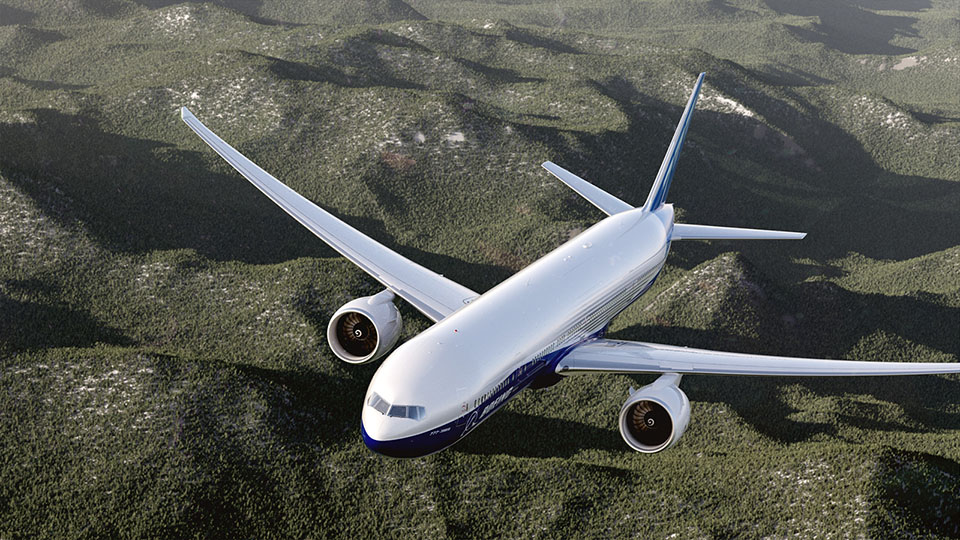
\includegraphics[width=1in]{img/plane-real.jpg}&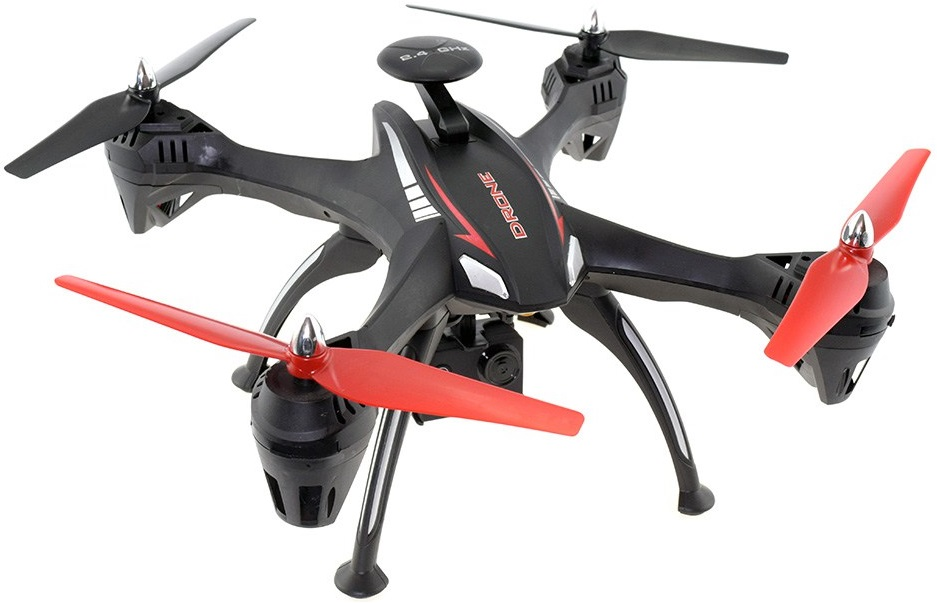
\includegraphics[width=1in]{img/quadcopter-real.jpg}&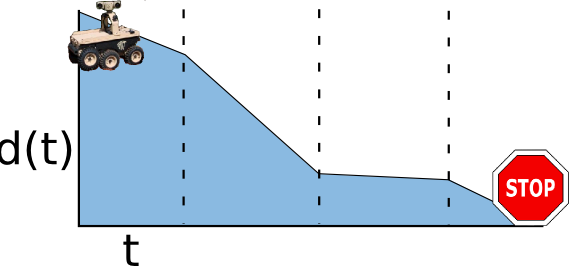
\includegraphics[width=1in]{img/robot-dyn-small.png}\\
%Planes&Drones&Robots\\
%\uncover<2->{
%& &\\
%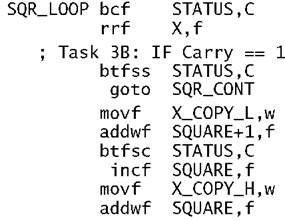
\includegraphics[width=0.6in]{img/assembly-small.png}&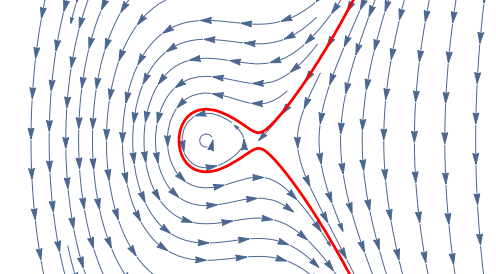
\includegraphics[width=1in]{img/invariant-region.png}&\infer{\Gamma \vdash A \lor B}{\Gamma \vdash A}\\
%Discrete Control & Continuous Dynamics & Syntactic Proof
%}
%    \end{tabular}
%  \end{center}
%  \only<1>{
%  \begin{quote}
%    How can we design cyber-physical systems people can bet their lives on? -- Jeanette Wing
%  \end{quote}
%  }
%  \only<3>{
%  \begin{quote}
%    How do proofs connect to reality?
%  \end{quote}
%  }
%\end{frame}


\begin{frame}[t]{Verification Needs to be End-to-end}
\begin{center}
  \begin{tabular}{lll}
% \acl{1}{Space shuttle}       & \acl{2}{40~\cite{DBLP:conf/cpsweek/ChanM17}}       & \acl{3}{400K}\\ % artifact provided: spaceex
% \acl{1}{Modern drone}        & \acl{2}{80~\cite{DBLP:conf/emsoft/RickettsML16}}   & \acl{3}{3M}\\
% \acl{1}{Pacemaker}           & \acl{2}{650~\cite{DBLP:conf/cpsweek/AndalamMRT16}} & \acl{3}{60K}  \\ % 35 cells * 19 lines
% Also: F22 ~> 1M lines, F35: 24M
\ah{1}{Application}         & \ah{2}{Models LOC (approx.)}                      & \ah{3}{Real system LOC} \\
\acl{1}{Insulin pump}        & \acl{2}{30~\cite{COBELLI198227}}                   & \acl{3}{35K~\cite{OpenAPS}}  \\ % number of equations in paper
\acl{1}{Commercial airliner} & \acl{2}{84-150~\cite{DBLP:conf/fm/PlatzerC09,DBLP:conf/emsoft/JeanninGKGSZP15}} & \acl{3}{14M~\cite{codebases}} \\  % tangential roundabout study, safe_explicit.kyx
\acl{1}{Modern car}          & \acl{2}{29-150~\cite{DBLP:conf/fm/LoosPN11,DBLP:journals/ral/BohrerTMSP19}}  & \acl{3}{100M~\cite{codebases}} %FM kym3 proof, 
  \end{tabular}
\end{center}
\end{frame}

\begin{frame}[t]{End-to-end Verification Must Close Several Gaps}
Why are implementations more complicated than models?
  \begin{align*}
%    \text{Non-critical code}  &\rightsquigarrow \langle\textbf{poof}\rangle
    \text{Learned Controls}     &\rightsquigarrow \text{Control envelopes}\\
    \text{Sensing + Actuation}  &\rightsquigarrow \text{Model assumptions}\\
    \text{Actual Physics}       &\rightsquigarrow \text{Diff.\ eq.}
  \end{align*}
\end{frame}

\begin{frame}[t]{End-to-end Verification Must Meet Competing Needs}
\begin{center}
  \begin{tabular}{lll}
    \ah{1}{\engineer} & \ah{2}{\logician} & \ah{3}{\logicuser}\\
    \acl{1}{Engineer} & \acl{2}{Logician} & \acl{3}{Logic-User}
  \end{tabular}
\end{center}
\end{frame}

%\section{Related Work}
%Also: Smooth out animation timing
%\begin{frame}[t]{General-purpose interactive theorem proving}
%  \begin{tabular}{lll}
%    \ah{1}{\engineer} & \ah{2}{\logician} & \ah{3}{\logicuser}\\
%    \acl{1}{\saySad{Generated code is \\hard to integrate}} & \acl{2}{\sayHappy{Strong Foundations!}} & \acl{3}{\saySad{Long Proofs!}}
%  \end{tabular}
%  \begin{itemize}
%  \item ROSCoq:~\cite{DBLP:conf/itp/AnandK15}            Coq proofs + control synthesis
%  \item VeriDrone:~\cite{DBLP:conf/emsoft/RickettsML16}  LTL in Coq + monitor synthesis
%  \item Isabelle/UTP:~\cite{DBLP:conf/utp/Foster19}      CPS Embedded in Isabelle
%  \end{itemize}
%\end{frame}

% \begin{frame}[t]{Model Checking + Synthesis}
%   \begin{tabular}{lll}
%     \ah{1}{\engineer} & \ah{2}{\logician} & \ah{3}{\logicuser}\\
%     \acl{1}{\sayHappy{Synthesis tools!}} & \acl{2}{\saySad{Paper foundations}} & \acl{3}{\saySad{Hard models!}}
%   \end{tabular}
%   \begin{itemize}
%   \item LTLMoP~\cite{DBLP:conf/iros/FinucaneJK10} and TuLiP~\cite{DBLP:conf/IEEEcca/FilippidisDLOM16}: Fancy front-end, synthesis via discretized model
%   \item \cite{DBLP:conf/rv/DesaiDS17}: Constant dynamics, STL-based runtime monitor
%   \item \cite{DBLP:conf/cdc/BhatiaKV10,DBLP:journals/automatica/FainekosGKP09}: Plan synthesis, complementary to control
%   \end{itemize}
% \end{frame}

% \begin{frame}[t]{\dL Verification + Synthesis (before)}
%   \begin{tabular}{lll}
%     \ah{1}{\engineer} & \ah{2}{\logician} & \ah{3}{\logicuser}\\
%     \acl{1}{\saySad{Limited synthesis}} & \acl{2}{\saySad{Paper foundations}} & \acl{3}{\saySad{Don't like tactics!}}
%   \end{tabular}
%   \begin{itemize}
%   \item Uniform substitution~\cite[\S35,\S40]{Church:1956} is foundation of differential dynamic logic (\dL)~\cite{DBLP:journals/jar/Platzer17}
%   \item \KeYmaeraX~\cite{DBLP:conf/cade/FultonMQVP15} prover uses Bellerophon~\cite{DBLP:conf/itp/FultonMBP17} language to express \dL proofs
%   \item \ModelPlex~\cite{DBLP:journals/fmsd/MitschP16} synthesizes correct-by-construction monitor conditions from \dL model
%   \end{itemize}
% \end{frame}

\begin{frame}[t]{No prior work meets all requirements}
\begin{table}[tbh]
  \centering
\begin{tabular}{l|c|c|r}
Approach    & Logician                 & Engineer                               & Logic-User\\\hline
GPITP       &\cellcolor{green!25}formal &\cellcolor{yellow!25}manual effort      &\cellcolor{orange!25}labor-intensive\\\hline
Automata    &\cellcolor{yellow!25}paper &\cellcolor{green!25}monitors, controls  &\cellcolor{orange!25}error-prone \\\hline
\dL before  &\cellcolor{yellow!25}paper &\cellcolor{yellow!25}some monitors      &\cellcolor{yellow!25}less error-prone\\\hline\pause       %, less labor-intensive
Current     &\cellcolor{green!25}formal &\cellcolor{yellow!25}some monitors      &\cellcolor{yellow!25}less error-prone\\\hline\pause %, less labor-intensive
Proposed    &\cellcolor{green!25}formal &\cellcolor{green!25}monitors, controls  &\cellcolor{green!25}least error-prone\\\hline       %, less labor-intensive
\end{tabular}
  \caption{Comparison of Verification Approaches}
  \label{tab:approach-comparison}
\end{table}
\end{frame}

\begin{frame}[t]{\CdGL Verification + Synthesis (after)}
  \begin{tabular}{@{\hskip0.6in}lll}
    \ah{1}{\engineer} & \ah{2}{\logician} & \ah{3}{\logicuser}\\
    \acl{1}{\sayHappy{Full synthesis suite!}} & \acl{2}{\sayHappy{Formal foundations!}} & \acl{3}{\sayHappy{Structured proofs!}}
  \end{tabular}
\begin{tabular}{@{\hskip-0.2in}l@{\hskip-0.7in}l}
\begin{minipage}{0.6\textwidth}
{\small\begin{itemize}
  \item[] \textbf{Complete:} Verified \dL checker
  \item[] \textbf{Complete:} Verified  monitor compilation
  \item[] \textbf{Complete:} Discrete-game logic
\end{itemize}}
\end{minipage} &
\begin{minipage}{0.6\textwidth}
{\small\begin{itemize}
  \item[] \textbf{In-progress:} Structured proofs
  \item[] \textbf{Proposed:} Synthesize monitor+control via
  \item[] \textbf{Proposed:} Hybrid-game logic
\end{itemize}}
\end{minipage}
\end{tabular}
\end{frame}


\section{Completed Work}
% Patter: We're now going to focus in on this thesis proper.
% First I'm going to discuss the completed works of the thesis, and for that I'm going to break
% down the thesis as a verification *pipeline*, as a series of steps in proof and implementation.
%
% Just to foreshadow: We will come back to the overview when I cover proposed work.
% The pipeline will be the same, rather the proposed work will achieve a better balance for our
% three characters within that pipeline.
\begin{frame}[t]{Approach of Thesis}
\begin{center}
  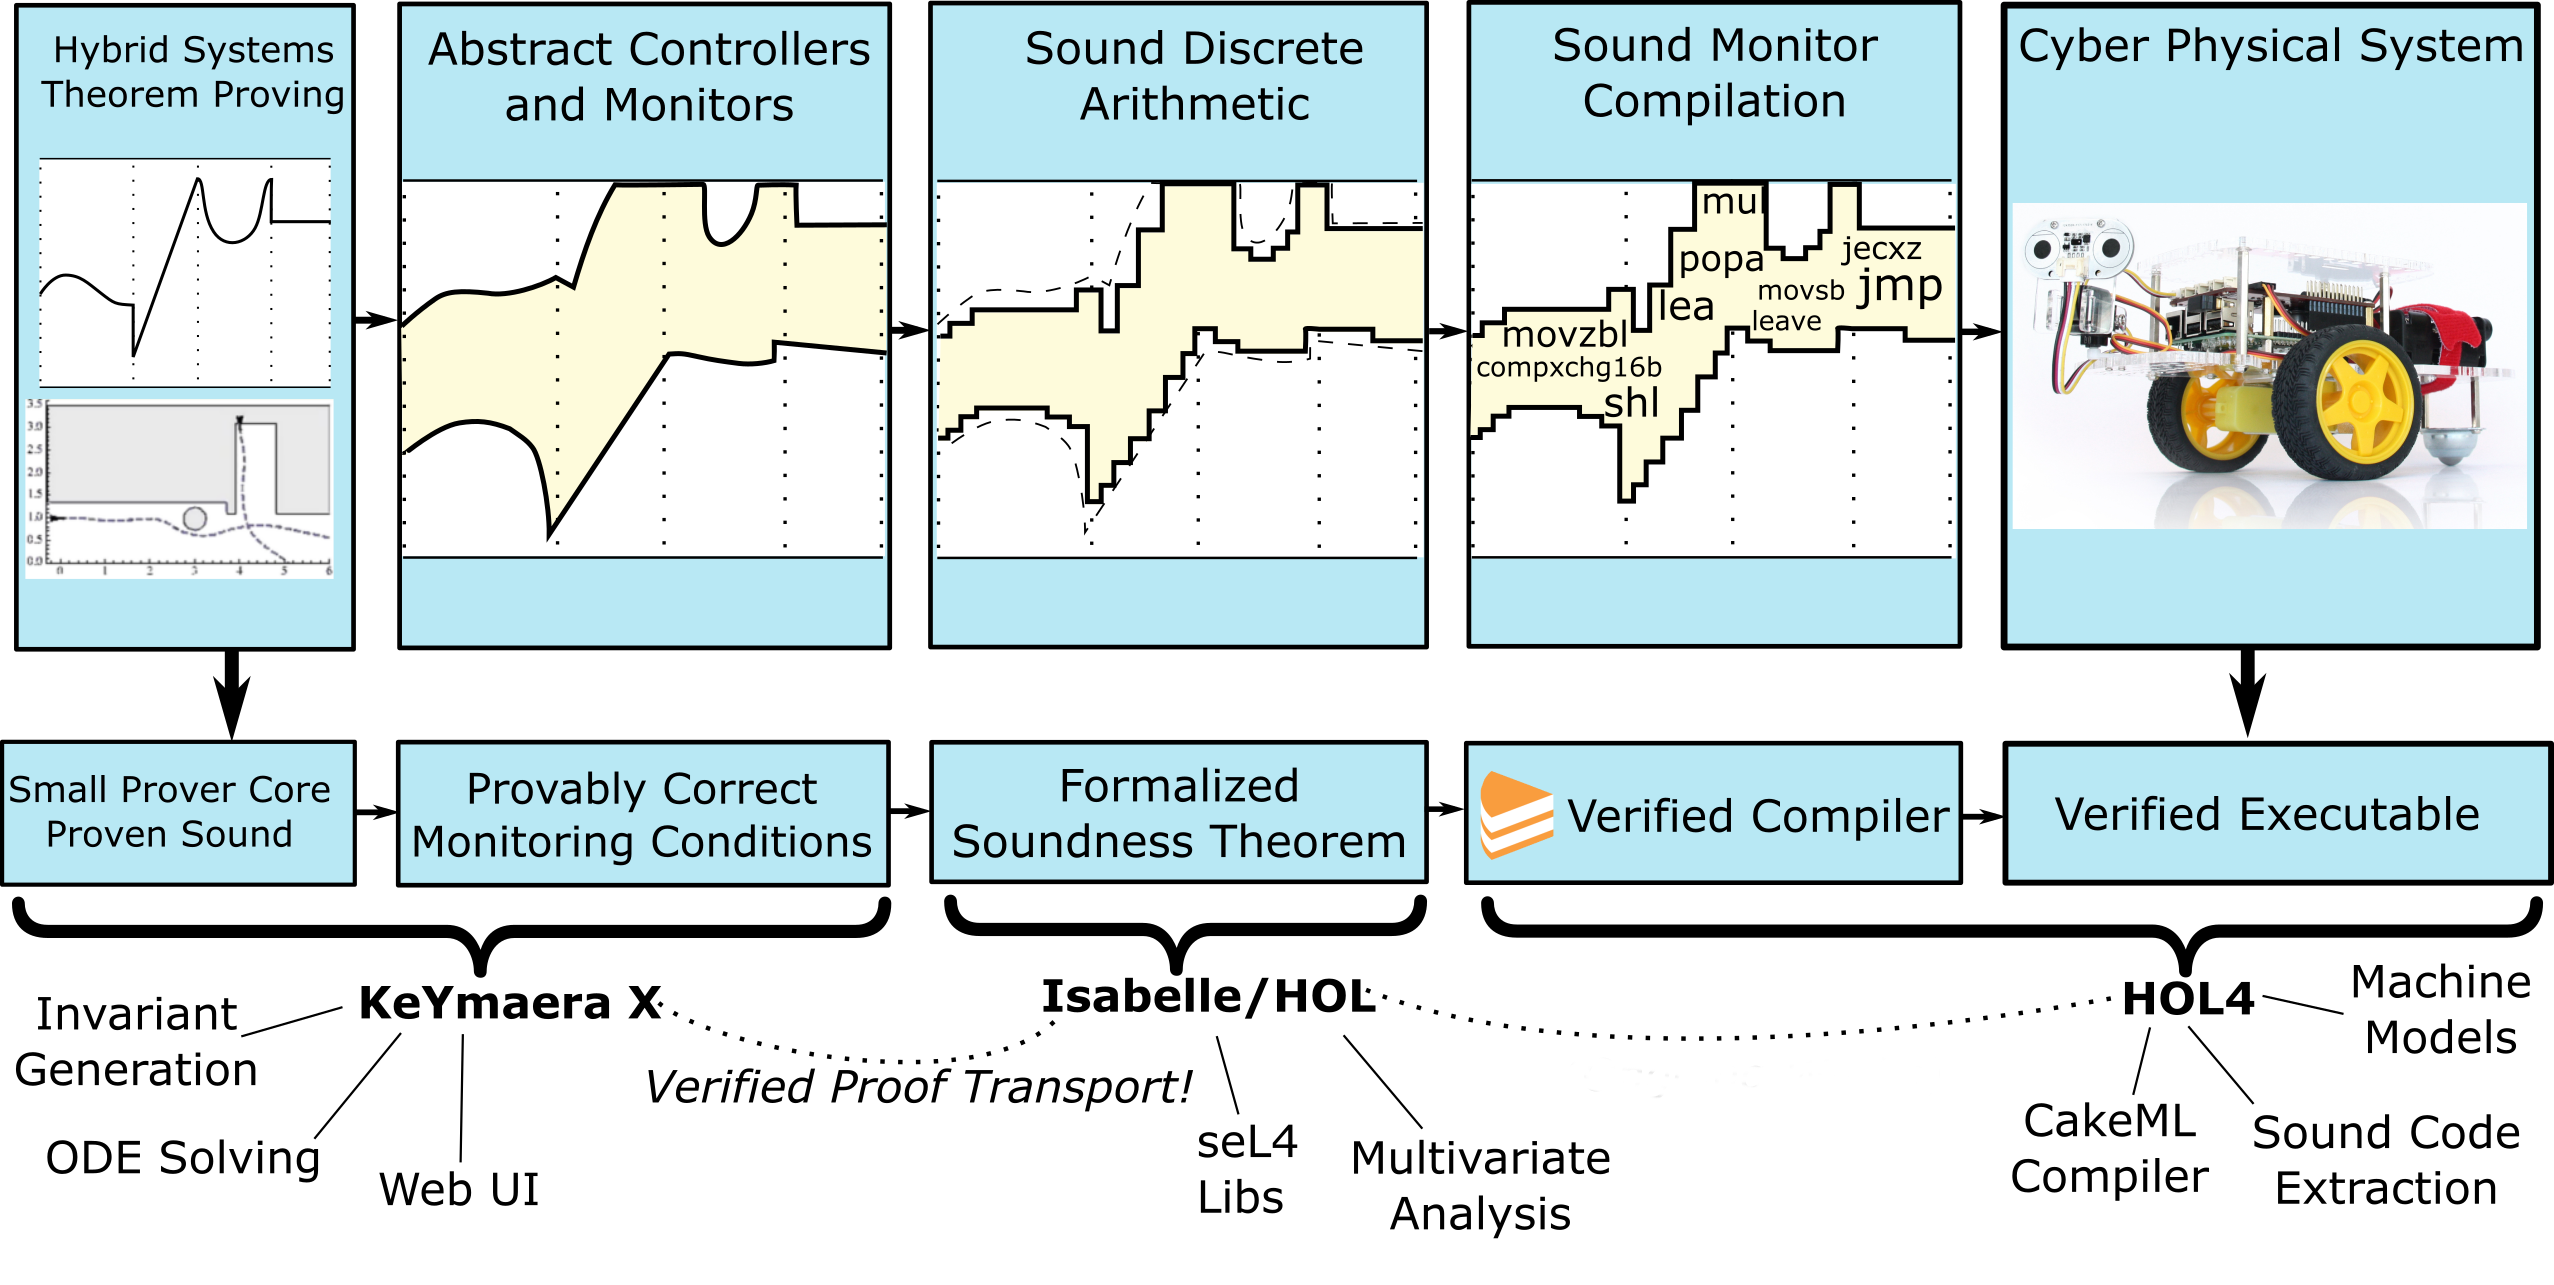
\includegraphics[width=4.4in]{img/veriphy-overview.png}
\end{center}
\end{frame}

\newcommand{\admiss}{\textsf{Go}}
\newcommand{\planreq}{\textsf{Feas}}
\newcommand{\veps}{\varepsilon}
\newcommand{\annul}{\textsf{Ann}\xspace}
\newcommand{\adjustSpeedDist}{\delta_\mathsf{Lim}\xspace}
\newcommand{\controllableGoalDist}{\mathsf{Lim}}
%\annul &~\mequiv~\abs{\kvar}\veps \leq 1 \land \Big|\frac{ \kvar~\left(\xgvar^2 +\ygvar^2 - \veps^2 \right)}{2} - \xgvar\Big| < \veps\\
%\label{eq:planReq} \planreq &~\equiv \annul \land \ygvar{>}0 \land 0{\leq}\vlvar{<}\vhvar \land \Avar\Tvar{\leq}\vhvar-\vlvar \land \Bvar\Tvar{\leq}\vhvar-\vlvar\\
%\admiss &\equiv a \in [-B,A] \land safe(v(a,\veps),x(a,\veps))\\
\begin{frame}{2D Driving Model is Input}
%\begin{tabular}{cc}
\noindent
\begin{minipage}{0.4\textwidth}
{\small\begin{align*}
\alpha~\equiv~& \prepeat{(\ctrl; \plant)}\\
\ctrl ~\equiv~& \prandom{\text{\sf{way,k,\m{v_{\text{lim}}}}}};\,\ptest{\planreq};\\
      &\underbrace{\prandom{\avar};\,\ptest{\admiss}}_{\ctrlliv}\\
\plant\equiv \{&\D{\xgvar}=-\vvar~\kvar~\ygvar,~\D{\ygvar}=\vvar~(\kvar~\xgvar-1),\\
             &~\D{\vvar}=\avar,~\D{\tvar}=1 \&~\tvar\leq \Tvar ~\land~ \vvar \geq 0\}
\end{align*}}
\end{minipage}%
\begin{minipage}{0.15\textwidth}~
\end{minipage}%
\begin{minipage}{0.45\textwidth}
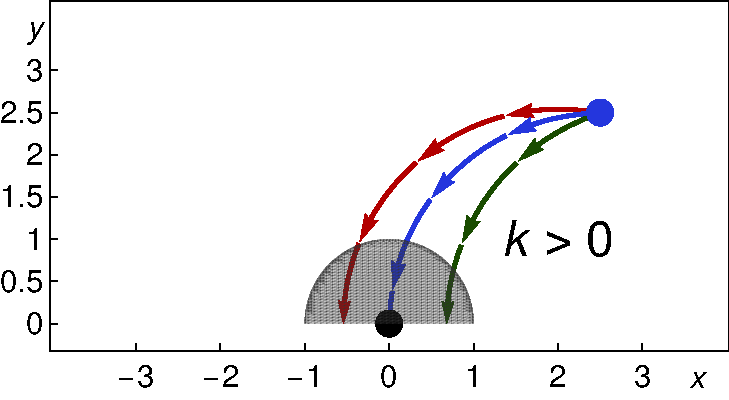
\includegraphics[width=\textwidth]{graphics/fig-ode2.pdf}
\end{minipage}
%\begin{minipage}{0.6\textwidth}
%\end{minipage}

%&
%\end{tabular}
\end{frame}

\begin{frame}[t]{Provable Monitor $\leadsto$ Provable Sandbox}
Sandboxed controller uses {\color{myyellow}{external}}  controller when decision is {\color{vred}safe}, else uses verified {\color{vgreen}{fallback}}.
Detects non-compliant {\color{vblue}plants}.
\begin{textblock}{8}(-0.5,4)
\footnotesize\begin{align*}
&\prandom{\vec{x}};\\
&\ptest{\phi}\\
& \bigl(\hspace{.5em} \color{myyellow}{\pumod{\vec{x}^+}{\textsf{extCtrl}}}\\
& \quad (~\phantom{\cup} \ptest{\color{vred}{\ctrlMon(\vec{x},\vec{x}^+)}}\\
& \quad \phantom{(~}\cup {\color{vgreen}{\fallback}} ~); \goback{}\\
& \quad \pumod{\vec{x}}{\vec{x}^+}\\
& \quad \prandom{\vec{x}^+} \\
& \quad  \ptest{\color{vblue}{\plantMon(\vec{x},\vec{x}^+)}};\\
& \quad  \pumod{\vec{x}}{\vec{x}^+}\bigr)^*
  \end{align*}
\end{textblock}
\begin{textblock}{10}(5,4)
\uncover<2->{
\scriptsize\begin{align*}
\textbt{fun}&~\texttt{cmlSandbox state =}\short
&\textbt{if}~\texttt{not ({\color{myyellow}stop ()}) }\textbt{then}\short
&\quad\texttt{state.ctrl}^+ \texttt{:= {\color{\extern}extCtrl state};}\short
&\quad\texttt{state.ctrl := }\textbt{if}\texttt{ {\color{vred}intervalSem ctrlMon state}} = \top \short
&\quad\quad\qquad\qquad\qquad\textbt{then}\texttt{ state.ctrl}^+\short
&\quad\quad\qquad\qquad\qquad\textbt{else}\texttt{ {\color{vgreen}fallback state;}}\short
&\quad\texttt{{\color{\extern}actuate state.ctrl};}\short
&\quad\texttt{state.sensors}^+\texttt{:= {\color{\extern}sense ()};}\short
&\quad\textbt{if}\texttt{ {\color{vblue}intervalSem plantMon state}} = \top\texttt{ }\textbt{then} \short
&\quad\quad\texttt{Runtime.fullGC ();} \short
&\quad\quad\texttt{state.sensors := state.sensors}^+\texttt{;} \short
&\quad\quad\texttt{cmlSandbox state} \short
&\quad\textbt{else}\texttt{ violation "Plant Violation"}
\end{align*}}
\end{textblock}
\begin{textblock}{20}(1.5,14)
\uncover<3->{
\noindent%
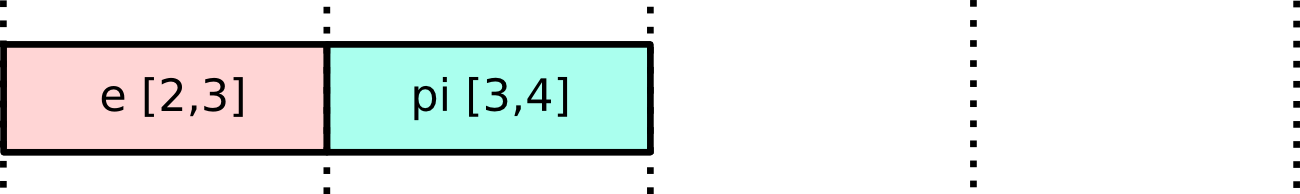
\includegraphics[width=1.6in]{img/interval1.png}\hskip0.4in%
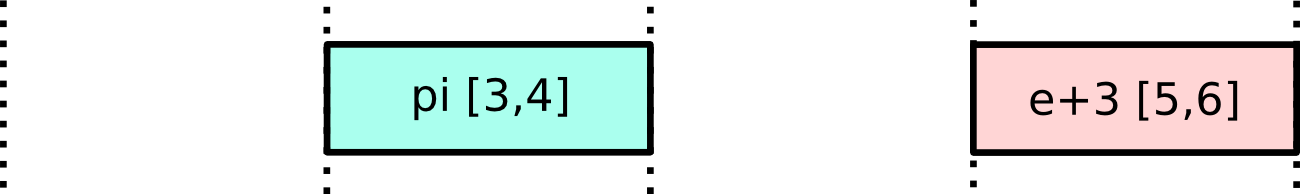
\includegraphics[width=1.6in]{img/interval2.png}\hskip0.4in%
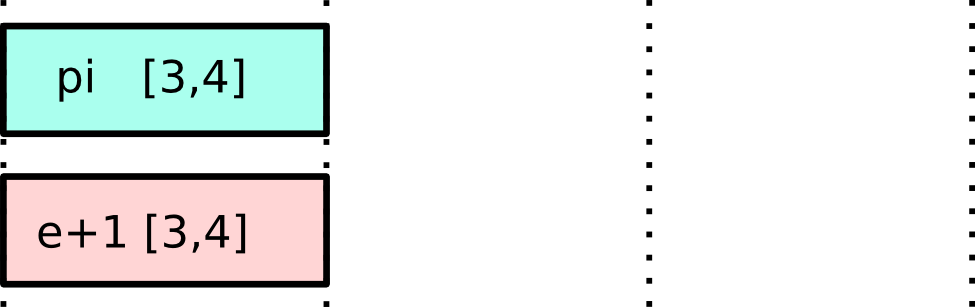
\includegraphics[width=1.1in]{img/interval3.png}}
\end{textblock}

%  \CakeML source incorporates {\color{myyellow}{external}} control, actuation, sensing
%\begin{textblock}{10}(5,3.5)
%%Note: Was cut for simplicity
%\small\begin{align*}
%& \prandom{V};~\prandom{\varepsilon};~ \prandom{d};~\prandom{t}; \goback{}\\
%& \ptest{d \geq 0 \land V\geq 0 \land \varepsilon \geq 0};  \goback{}\\
%& \bigl(\hspace{.5em} \color{myyellow}{\prandom{t^+};~\prandom{v^+};~ \pumod{d^+}{d};}  \goback{}\\
%& \quad (~\phantom{\cup} \ptest{\color{vred}{\ctrlMon(d,t,v,d^+,t^+,v^+)}}\\
%& \quad \phantom{(~}\cup \color{vgreen}{\pumod{t^+}{0};~\pumod{v^+}{0}} ~); \goback{}\\
%& \quad \pumod{t}{t^+};~\pumod{v}{v^+};  \goback{}\\
%& \quad  \prandom{d^+};~\prandom{t^+};  \goback{}\\
%& \quad  \ptest{\color{vblue}{\plantMon(d,t,v,d^+,t^+,v^+)}};\\
%& \quad  \pumod{d}{d^+};~\pumod{t}{t^+}  \goback{}\bigr)^* 
%\end{align*}
%\end{textblock}
\end{frame}

\begin{frame}[t]{Verified Proof Term Checker}
Proof checker formalized as function:
\[{\tt pteval} : {\tt pt} \to {\tt proofState\ option}\]\pause
Soundness theorem formalized:
\[\small\texttt{arith\_valid pt} \land \texttt{pteval\ pt = Some rule} \limply \texttt{sound(rule)}\]\pause
Tested on real sandbox proofs ($\approx$100,000 steps)
\end{frame}
%How to trust a theorem prover?
%Formalize it!
%\Isabelle function \texttt{pteval} computes the proof state proved by a given proof term, or returns \texttt{NONE} on proofs that do not check
%\KeYmaeraX is instrumented with a proofterm checker.
%The synthesized checker was evaluated on a 100,000-step sandbox safety proof.
%Decidable first-order arithmetic is assumed ``axiomatically,'' all other rules are proven sound.
%\begin{theorem}[Proof-checker soundness]
%If all real arithmetic subgoals are valid and the proof checker accepts the proof term, the output derived rule is sound, i.e.:
%\end{theorem}


%\begin{frame}{Sandbox is Discretized}
%\textbf{Example:} Check whether $\pi < e$, efficiently.\\
%\textbf{Solution:} Conservative interval approximation
%\begin{example}
%Let $\nu_I=\{pi\mapsto[3,4],e\mapsto[2,3]\}$, then 
%\begin{itemize}
%%%%\item<+-> \(pi <_w e\) is false ($\bot$)\hspace{1.16in}\includegraphics[width=1.5in]{img/}
%\item<+-> \(pi <_w e\) is false ($\bot$)\hspace{1.63in}
%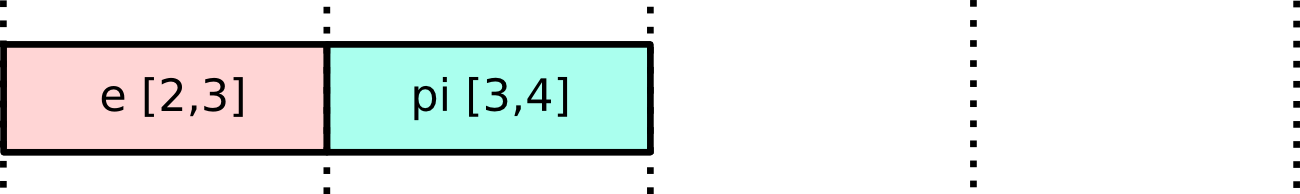
\includegraphics[width=1.875in]{img/interval1.png}
%\item<+-> \(pi <_w e + 3\) is true ($\top$)\hspace{1.4in}
%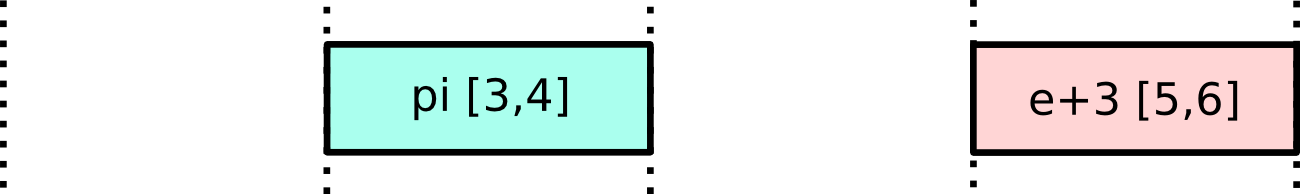
\includegraphics[width=1.875in]{img/interval2.png}
%\item<+-> \(pi <_w e + 1\) is \emph{a known unknown} ($U$){\hspace{0.50875in}
%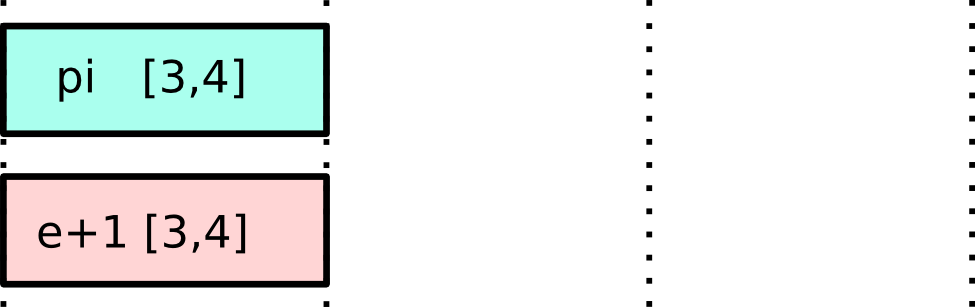
\includegraphics[width=1.40625in]{img/interval3.png}
%}
%\end{itemize}
%\only<4>{When truth values can be unknown, resulting logic is \emph{3-valued}}
%\end{example}
%\begin{textblock}{10}(14,1.75)
%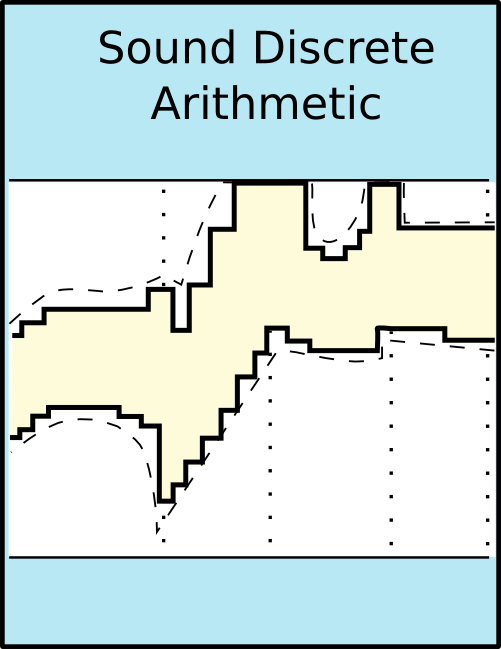
\includegraphics[width=0.7in]{img/focus-int.png}
%\end{textblock}
%\end{frame}

%\begin{frame}[t]{Discrete Sandbox is Compiled}
%\end{frame}

\begin{frame}[t]{Compiled Code is Simulated}
\begin{figure}[tb]
\centering
\begin{minipage}[b]{2in}\centering
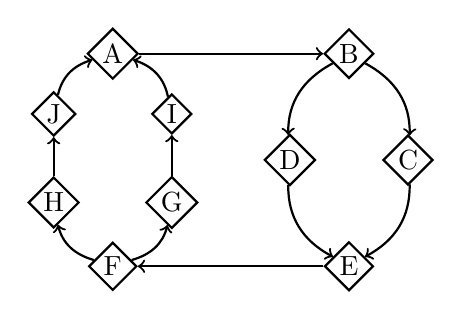
\begin{tikzpicture}[->,draw,thick,yscale=0.9,inner sep=1pt]
\tikzstyle{arc}=[circle,draw]
\tikzstyle{line}=[rectangle,draw]
\tikzstyle{way}=[diamond,draw]
\node[way] (a) at (1,3) {A};
\node[way] (b) at (4,3) {B};
\node[way] (c) at (4.75,1.5) {C};
\node[way] (d) at (3.25,1.5) {D};
\node[way] (e) at (4,0) {E};
\node[way] (f) at (1,0) {F};
\node[way] (g) at (1.75,0.90) {G};
\node[way] (h) at (0.25,0.90) {H};
\node[way] (i) at (1.75,2.15) {I};
\node[way] (j) at (0.25,2.15) {J};
\draw (a) -> (b);
\draw (b) edge [bend left] node {} (c);
\draw (b) edge [bend right] node {} (d);
\draw (c) edge [bend left]node {} (e);
\draw (d) edge [bend right] node {} (e);
\draw (e) -> (f);
\draw (f) edge [bend left]  node {} (h);
\draw (f) edge [bend right] node {} (g);
\draw (h) -> (j);
\draw (g) -> (i);
\draw (j) edge [bend left]  node {} (a);
\draw (i) edge [bend right] node {} (a);
\end{tikzpicture}
\subcaption{Example mission}\label{fig:patrol-mission-plan}\end{minipage}
\begin{minipage}[b]{1.51in}\centering
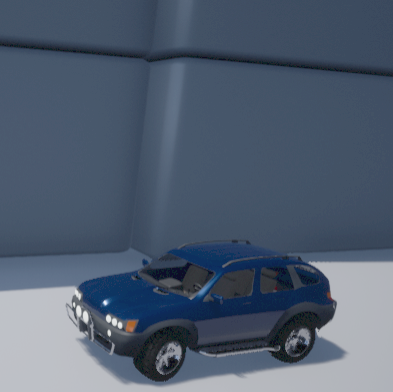
\includegraphics[width=1.51in,clip,trim=0 0 0 50]{graphics/airsim.png}
\subcaption{Simulator}\label{fig:simulator}\end{minipage}
\begin{minipage}[b]{1in}\centering
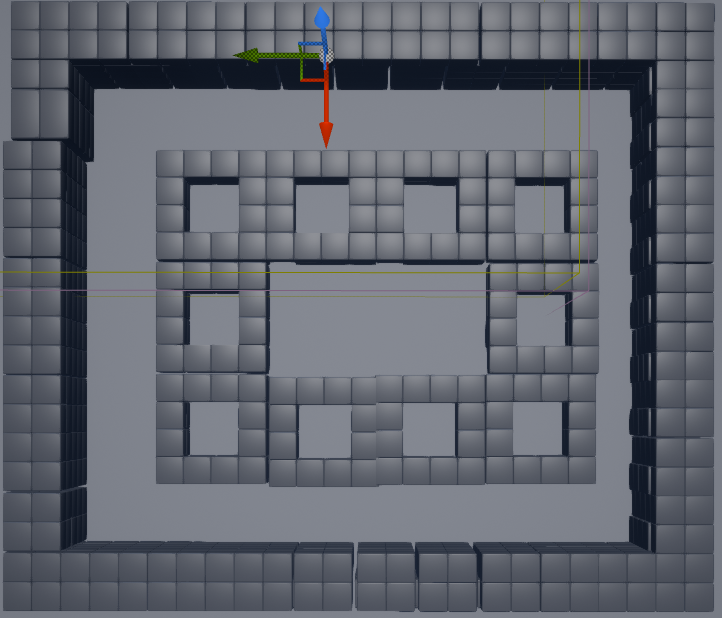
\includegraphics[width=1in]{graphics/screen1.png}
\subcaption{Rectangle}\label{fig:rect}\end{minipage}\\
\begin{minipage}[b]{1in}\centering
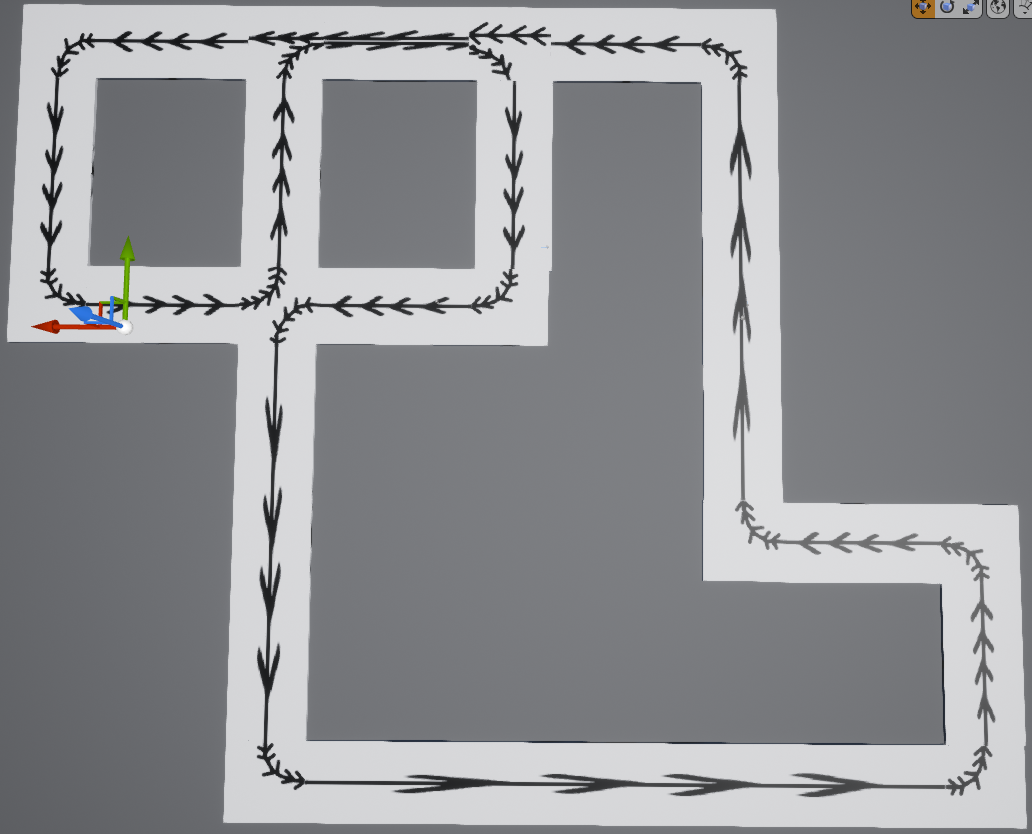
\includegraphics[width=1in]{graphics/screen2.png}
\subcaption{Tight turns}\label{fig:turns}\end{minipage}
\begin{minipage}[b]{1in}\centering
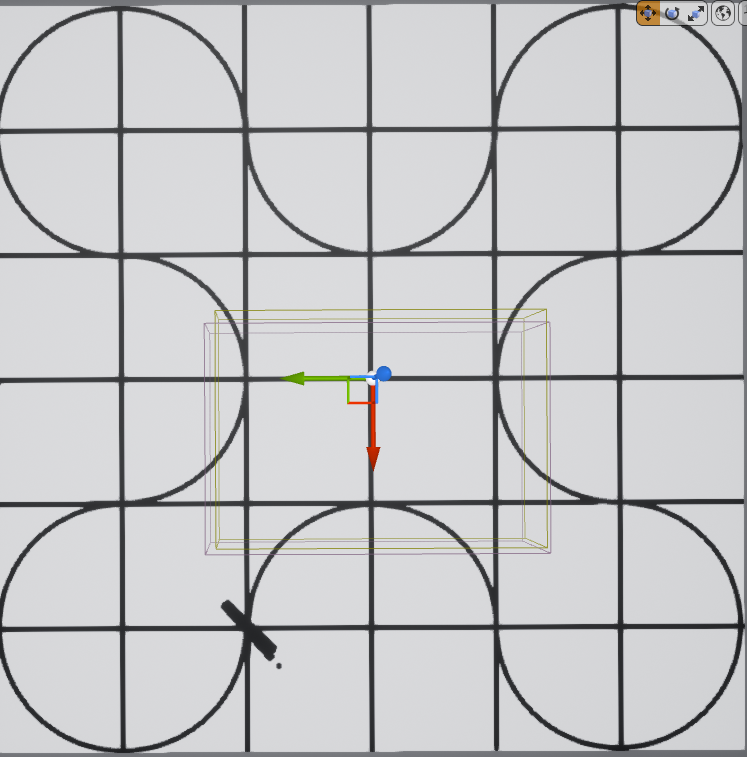
\includegraphics[width=0.8in]{graphics/screen3.png}
\subcaption{Large clover}\label{fig:clover}\end{minipage}
\caption{Implementation and environments built in AirSim}
\label{fig:patrol-plan}
\end{figure}
\end{frame}


\begin{frame}[t]{Components of Thesis}
\newcommand{\cdone}{green!10}
\newcommand{\cwip}{yellow!30}
\newcommand{\cprop}{orange!30}
%\begin{center}
\noindent\hskip-0.2in
\begin{tikzpicture}[scale=0.5]
\draw (0,3.2)  node {Logic for};
\draw (0,2.4)  node {Hybrid Systems};
\draw (0,0)   node[circle]      (CdGLcirc) {\phantom{\hspace{1.1cm}}};
\draw (0,-1) node (cdgl) {\phantom{\CdGL}};
\node[coordinate,pin={[pin distance=0.55cm,text width=2cm]320:{\S6}}] (cdgl-ref) at (cdgl) {};
\draw (0,0)   node[circle, fill=red!20,draw]      (CdGLcirc) {\phantom{\hspace{1.6cm}}};
\draw (0,-1.2) node (cdgl) {\CdGL};
\draw (0,0)   node[circle]  (dl)  {\phantom{\dL}};
\node[coordinate,pin={[pin distance=0.9cm,text width=3cm]265:{\ \ \ \ \ \ \ \ \ \S3 \S4}}] (dl-ref) at (dl) {};
\draw (dl) node[circle, fill=blue!20,draw]  {\dL};
\draw (-7, 1.3) node[rectangle,rounded corners,fill=green!20,draw,text depth=1in,text width=1.2in,text centered] (logic) {Foundations};
\draw (-7, 2.8) node[rectangle,rounded corners,fill=\cdone,draw,thin,minimum height=0.3cm] (formalization) {\dL Formalized};
\draw (-7, 1.7) node[rectangle,rounded corners,fill=\cdone,draw,thin,minimum height=0.3cm] (generalization) {\color{vgray}\dL Generalized};
\draw (-14,1.7) node {{\small\color{vgray}Not in Talk}};
\draw (-7, 0.6) node[rectangle,rounded corners,fill=\cwip,draw,thin,minimum height=0.3cm] (cgl) {Constructive \GL};
\draw (-7, -0.5) node[rectangle,rounded corners,fill=\cprop,draw,thin,minimum height=0.3cm] (cdgl) {Constructive \dGL};
\draw node[left=0.3cm of formalization] (formal-ref) {\S3.1};
\draw node[left=0.3cm of generalization] (gen-ref) {\S3.2};
\draw node[left=0.3cm of cgl] (cgl-ref) {\S5};
\draw node[left=0.3cm of cdgl] (cdgl-ref) {\S6};
\draw[dashed] (formalization) -- (formal-ref);
\draw[dashed] (generalization) -- (gen-ref);
%2.6
\draw (5, 1.4) node[rectangle,rounded corners,fill=green!20,draw,text depth=1in,text width=2.1cm,text centered] (engine) {Artifacts};
\draw (5, 2.6) node[rectangle,rounded corners,fill=\cdone,draw,thin,minimum height=0.3cm] (proofterm) {Proof Term};
\draw (5, 1.4) node[rectangle,rounded corners,fill=\cdone,draw,thin,minimum height=0.3cm] (monitors) {Monitors};
\draw (5, 0.2) node[rectangle,rounded corners,fill=\cwip,draw,thin,minimum height=0.3cm] (proofscript) {Proof Script};
\draw (5, -1) node[rectangle,rounded corners,fill=\cprop,draw,thin,minimum height=0.3cm] (controllers) {Controls};
\draw node[right=0.3cm of monitors] (monitor-ref) {\S4.1};
\draw node[right=0.3cm of controllers] (controllers-ref) {\S8};
\draw node[right=0.3cm of proofscript] (proofscript-ref) {\S7};
\draw node[right=0.3cm of proofterm] (proofterm-ref) {\S4.1};
\draw[dashed] (monitors) -- (monitor-ref);
\draw[dashed] (controllers) -- (controllers-ref);
\draw[dashed] (proofscript) -- (proofscript-ref);
\draw[dashed] (proofterm) -- (proofterm-ref);
\node[shape=coordinate] (use-anchor) at (0,-3){};
\draw (0, -5.1) node[rectangle,rounded corners,fill=green!20,draw,text depth=1.6cm,text width=2.1in,text centered] (luser) {Usability};
\draw (0.3, -4.7) node[rectangle,rounded corners,fill=\cprop,draw,thin,minimum height=0.3cm] (monitors)    {Simplicity};
\draw (0.1, -4.7) node[rectangle,rounded corners,fill=\cprop,draw,thin,minimum height=0.3cm,text width=4.8cm] (lop)    {Lines of Model/Proof};
\draw (-2.9, -6.05) node[rectangle,rounded corners,fill=\cprop,draw,thin,minimum height=0.3cm,text width=2cm] (modelmistake) {Model Bugs};
\draw (2.4, -6) node[rectangle,rounded corners,fill=\cprop,draw,thin,minimum height=0.3cm,text width=2.4cm] (maintainable) {Maintainable?};
\draw node[right=0.3cm of maintainable] (maintain-ref) {\S7};
\draw node[right=0.3cm of lop] (lop-ref) {\S7};
\draw[->,very thick] (logic) -- (CdGLcirc);
\draw[->,very thick] (CdGLcirc) -- (engine);
\draw[dashed] (CdGLcirc) -- (luser);
\draw[dashed] (lop) -- (lop-ref);
\draw[dashed] (maintainable) -- (maintain-ref);
%\draw (1.45,-2) -- (0,-2.7);
%\draw (0, -3.1) node[rectangle,rounded corners,fill=\cdone,draw,thin,minimum height=0.3cm] (monitors)    {Simplicity};
%\draw (0, -4.15) node[rectangle,rounded corners,fill=\cdone,draw,thin,minimum height=0.3in,text width=0.7in] (controllers) {Modeling Mistakes};
\end{tikzpicture}
%\end{center}
\end{frame}
%{\small\begin{align*}
%\ctrl &~\equiv~ \prandom{(\xgvar,\ygvar)};\,\prandom{[\vlvar,\vhvar]};\,\prandom{\kvar};\,\ptest{\planreq};\,\underbrace{\prandom{\avar};\,\ptest{\admiss}}_{\ctrlliv}\\
%\annul &~\mequiv~\abs{\kvar}\veps \leq 1 \land \Big|\frac{ \kvar~\left(\xgvar^2 +\ygvar^2 - \veps^2 \right)}{2} - \xgvar\Big| < \veps\\
%\label{eq:planReq} \planreq &~\equiv \annul \land \ygvar{>}0 \land 0{\leq}\vlvar{<}\vhvar \land \Avar\Tvar{\leq}\vhvar-\vlvar \land \Bvar\Tvar{\leq}\vhvar-\vlvar\\
%\admiss &\equiv a \in [-B,A] \land safe(v(a,\veps),x(a,\veps))\\
%\plant\equiv \{&\D{\xgvar}=-\vvar~\kvar~\ygvar,~\D{\ygvar}=\vvar~(\kvar~\xgvar-1),~\D{\vvar}=\avar,~\D{\tvar}=1 \\
% &\&~\tvar\leq \Tvar ~\land~ \vvar \geq 0\}
%\end{align*}}

\newcommand{\moncolor}[1]{\plantcolor{#1}}
\section{Ongoing Work: \CdGL Logic}
% Say: CGL is already done, but for the sake of time we're presenting it together with CdGL
\begin{frame}[t]{\only<1>{Diamonds Support Synthesis}\only<2>{Games Extend Systems}}
\begin{center}
  \begin{tikzpicture}
    \draw (0,1) node (thm) {$\dbox{\moncolor{\prandom{\vec{x}};\ptest{\planreq};}\ctrlcolor{\prandom{\avar};\ptest{\admiss}};\moncolor{\plant}}{\textsf{goal}}$};
    \draw (0,0.5) node {$\Uparrow$};
    \draw (0,0) node (mainprf) {$\dbox{\moncolor{\prandom{\vec{x}};\ptest{\planreq}}}{\ddiamond{\ctrlcolor{\prandom{\avar}}}{\dbox{\moncolor{\plant}}{\textsf{goal}}}}$};
    \draw (0,-0.5) node {\only<2>{$\Uparrow$}};
    \draw (0,-1) node (nxtprf) {\only<2>{$\dbox{\moncolor{\prandom{\vec{x}};\ptest{\planreq}};\ctrlcolor{\pdual{(\prandom{\avar})}};\moncolor{\plant}}{\textsf{goal}}$}};
    \draw (3.2,0.5) node {\footnotesize{\color{gray}Existential Simplification} (\ctrlcolor{$\admiss$} is $\approx$1 slide!)};
    \draw (1.7,-0.5) node {\only<2>{\footnotesize{\color{gray}Games Add Duality}}};
  \end{tikzpicture}
\end{center}
\end{frame}
%\begin{frame}[t]{Exploit Proof Content}
%  $J(x) \limply \ddiamond{\overline{\ctrlcolor{\ctrl}}}{\dbox{\plantcolor{\overline{\plant}}}{J(y<x)}}$
% $J(x) \limply \ddiamond{\ctrlcolor{\ctrl}}{\dbox{\plantcolor{\plant}}{J(y<x)}}$
%    \draw (0.6,0.5) node {\footnotesize{\color{gray}Proof}};
%    \draw (1.1,-0.5) node {\footnotesize{\color{gray}Elaboration}};
%    \draw (3, -0.5) node {\plantcolor{dC}};
%    \draw (3.15, -1) node {\plantcolor{dI}};
%    \draw (3, -1.5) node {\plantcolor{dG}};
%    \draw (4.7, -1) node {\plantcolor{\texttt{Plant.S}}};

%    \draw[color=vblue] (3.3, -0.5) -- (3.85,-0.85);
%    \draw[color=vblue] (3.4, -1)   -- (3.9,-1);
%    \draw[color=vblue] (3.3, -1.5) -- (3.85,-1.15);

%    \draw (-3, -0.5) node {\ctrlcolor{$\langle{'}\rangle$}};
%    \draw (-3, -1) node {\ctrlcolor{$\langle{:}{*}\rangle$}};
%    \draw (-3, -1.5) node {\ctrlcolor{$\langle{\cup}\rangle$}};
%    \draw (-5, -1) node {\ctrlcolor{\texttt{Control.S}}};

%    \draw[color=vred] (-3.5, -0.5) -- (-3.85,-0.85);
%    \draw[color=vred] (-3.4, -1)   -- (-3.9,-1);
%    \draw[color=vred] (-3.5, -1.5) -- (-3.85,-1.15);

%  \begin{tabular}{ccc}
%    Modality                  & Curry-Howard & Synthesizes \\
%    $\dbox{\alpha}{\phi}$     & Demon strategy for $\phi$ after $\alpha$ & Monitor \\
%    $\ddiamond{\alpha}{\phi}$ & Angel strategy for $\phi$ after $\alpha$ & Control
%  \end{tabular}\pause
%  \begin{itemize}
%  \item Games support monitor \emph{and} control synthesis from \emph{one} proof
%  \item Curry Howard foundation promotes general-case, robust tools
%  \item Game models are often simpler than systems
%  \end{itemize}

% Formula language, game language by Nim example, example properties
% Realizers, semantics
% quick 1-slide "proof terms exist"
% Soundness, prog+pres, implications for practice
% What's next: ODE's
\begin{frame}[t]{Systems Driving Model Exists}
\noindent
\begin{minipage}{0.4\textwidth}
{\small\begin{align*}
\ctrl ~\equiv~& \prandom{\text{\sf{way,k,\m{v_{\text{lim}}}}}};\,\ptest{\planreq};\\
      &\ctrlcolor{\prandom{\avar};\,\ptest{\admiss}}\\
\plant\equiv \{&\D{\xgvar}=-\vvar~\kvar~\ygvar,~\D{\ygvar}=\vvar~(\kvar~\xgvar-1),\\
             &~\D{\vvar}=\avar,~\D{\tvar}=1 \&~\tvar\leq \Tvar ~\land~ \vvar \geq 0\}
\end{align*}}%
\end{minipage}%
  \begin{minipage}{0.15\textwidth}~\end{minipage}%
\begin{minipage}{0.45\textwidth}
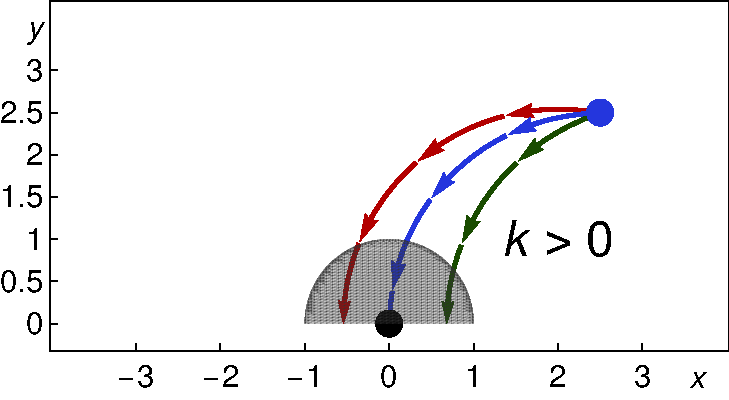
\includegraphics[width=2.3in]{graphics/fig-ode2.pdf}
\end{minipage}%
\end{frame}

\begin{frame}[t]{Game Model is Proposed}
%\begin{frame}[t]{2D Driving Model is Input}
%\begin{tabular}{cc}
\noindent
\begin{minipage}{0.4\textwidth}
{\small\begin{align*}
\ctrl ~\equiv~& \prandom{\text{\sf{way,k,\m{v_{\text{lim}}}}}};\,\ptest{\planreq};\\
      &\ctrlcolor{\pdual{\prandom{\avar}}}\\
\plant\equiv \{&\D{\xgvar}=-\vvar~\kvar~\ygvar,~\D{\ygvar}=\vvar~(\kvar~\xgvar-1),\\
             &~\D{\vvar}=\avar,~\D{\tvar}=1 \&~\tvar\leq \Tvar ~\land~ \vvar \geq 0\}
\end{align*}}%
\end{minipage}%
\begin{minipage}{0.15\textwidth}~\end{minipage}%
\begin{minipage}{0.45\textwidth}
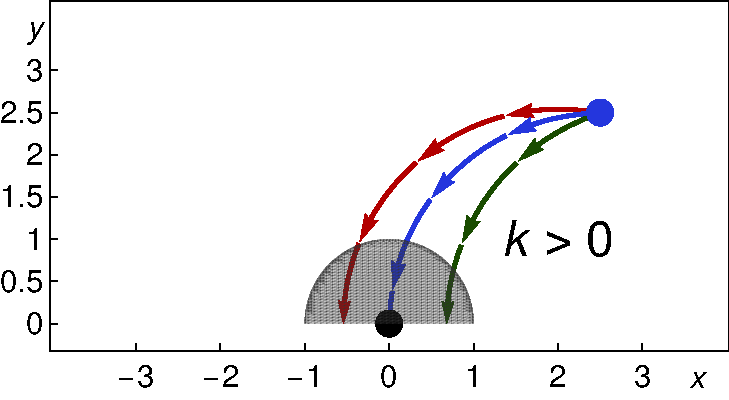
\includegraphics[width=2.3in]{graphics/fig-ode2.pdf}
\end{minipage}%
\end{frame}
\begin{frame}[t]{Game Model is Proposed}
\noindent
\begin{minipage}{0.4\textwidth}
{\small\begin{align*}
\ctrl ~\equiv~& \prandom{\text{\sf{way,k,\m{v_{\text{lim}}}}}};\,\ptest{\planreq};\\
      &\ctrlcolor{\pdual{\prandom{\avar}}}\\
\plant\equiv \{&\D{\xgvar}=-\vvar~\kvar~\ygvar,~\D{\ygvar}=\vvar~(\kvar~\xgvar-1),\\
             &~\D{\vvar}=\avar,~\D{\tvar}=1 \&~\tvar\leq \Tvar ~\land~ \vvar \geq 0\}
\end{align*}}%
\end{minipage}%
\begin{minipage}{0.15\textwidth}~\end{minipage}%
\begin{minipage}{0.45\textwidth}
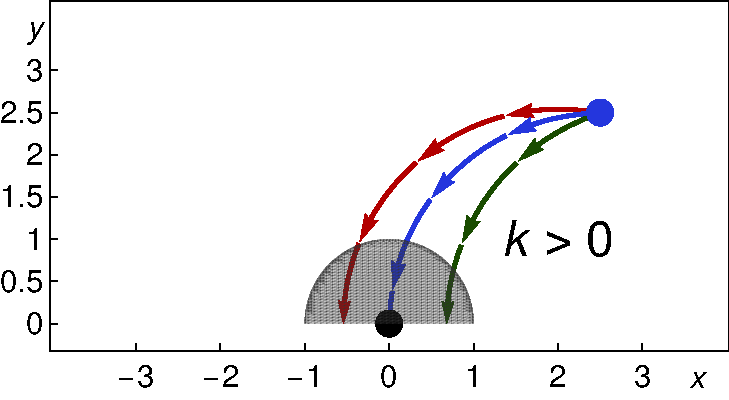
\includegraphics[width=2.3in]{graphics/fig-ode2.pdf}
\end{minipage}%
\begin{center}
\begin{align*}
\uncover<1->{\textsf{Live}} &\uncover<1->{\equiv \dbox{\drepeat{(\ctrl;\plant)}}{\textsf{goal}}}\\
\uncover<1->{\textsf{Safe}} &\uncover<1->{\equiv \ddiamond{\prepeat{(\ctrl;\plant)}}{\textsf{safe}}}\\%
\only<1>{\phantom{\textsf{Win}}  &\phantom{\equiv \ddiamond{\prepeat{(\ctrl;\plant;\ptest{\textsf{safe}})}}{\textsf{goal}}}}%
\only<2>{\textsf{Win}  &\equiv \ddiamond{\prepeat{(\ctrl;\plant;\ptest{\textsf{safe}})}}{\textsf{goal}}}%
\end{align*}
\end{center}
\end{frame}

\begin{frame}[t]{Realizers are Computable Strategies}
  \begin{align*}
\aa,\ab,\ac
&\bebecomes f  \alternative \rzBLam{x}{\tau}{\aa} \alternative \rzApp{\aa}{\ab} \alternative  \rzNil \alternative \rzCons{\aa}{\ab}  \alternative \rzFst{\aa} \alternative \rzSnd{\aa}
  \end{align*}
\begin{itemize}
\item Abstract base language $f$
\item Higher-order functions and tupling
\item Think: Calculus of Inductive Constructions (dependent $\lambda$-calculus)
\end{itemize}
\end{frame}

\begin{frame}[t]{Formula Semantics}
Which \emph{region} $X$ of strategy-state pairs $(\aa,\om)$ realizes $\phi$?
\[(\rzNil,\om) \in  \fintR{f \geq g} \text{ iff } \tint{f}{\om} \geq \tint{g}{\om}\]
Starting from region $X$, where does $\alpha$ take Angel?
\[(\aa,\om) \in  \fintR{\ddiamond{\alpha}{\phi}} \text{ iff } \strategyforR[\alpha]{\{(\aa,\om)\}} \subseteq (\fintR{\phi} \cup \{\stt\})\]
Starting from region $X$, where does $\alpha$ take Demon?
\[(\aa,\om) \in  \fintR{\dbox{\alpha}{\phi}} \text{ iff } \dstrategyforR[\alpha]{\{(\aa,\om)\}} \subseteq (\fintR{\phi} \cup \{\stt\})\]\pause
``Continuation passing semantics"
\end{frame}

% Patter: In random assignments, the computational content is "how do I compute this variable"
% In nondet choices the content is "how do I compute which branch to take"
% Likewise we can do all the cases but 45 minute talk
\begin{frame}[t]{Angel Game Semantics}
\begin{align*}
\strategyforR[\prandom{x}]{X}          &= \{(\rzSnd{\aa},\ssub{\om}{x}{\rzFst{\aa}(\om)})~|~(\aa,\om) \in X\}&&\text{}\\
\uncover<2->{\strategyforR[\alpha\cup\beta]{X}      &= \strategyforR[\alpha]{\apL{X}} \cup \strategyforR[\beta]{\apR{X}}&&\text{}\\}
\uncover<3->{\strategyforR[\ptest{\phi}]{X}            &= \{(\rzSnd{\aa},\om)~|~ (\aa,\om) \in X,~(\rzFst{\aa},\om) \in \fintR{\phi}\}\\
                                          &\cup \{\sff~|~(\aa,\om) \in X,~(\rzFst{\aa},\om) \notin \fintR{\phi}\}\\
\strategyforR[\humod{x}{f}]{X}  &= \{(\aa,\ssub{\om}{x}{\tint{f}{\om}})~|~(\aa,\om) \in X\}&&\text{}\\
\strategyforR[\alpha;\beta]{X}           &= \strategyforR[\beta]{(\strategyforR[\alpha]{X})} &&\text{}\\
\strategyforR[\prepeat{\alpha}]{X}     &= \bigcap\{\apL{Z}\subseteq \allRz \times \allstate~|~ X \cup (\strategyforR[\alpha]{\apR{Z}}) \subseteq Z\}
&&\\
\strategyforR[\pdual{\alpha}]{X}        &= (\dstrategyforR[\alpha]{X})&&\text{}}
\end{align*}
\end{frame}

\begin{frame}[t]{Games Support Proof Terms}
\[M,N \bebecomes \edcase{A}{B}{C} \alternative \edinjL{A} \alternative \cdots \] % \ebcons{A}{B}
\pause
\cinferenceRule[dchoiceE|{$\langle\cup\rangle${E}}]{}
{
\linferenceRule[formula]
{\proves{\G}{A}{\ddiamond{\alpha\cup\beta}{\phi}}
        &\proves{\G,\pvl:\ddiamond{\alpha}{\phi}}{B}{\psi}
        &\proves{\G,\pvr:\ddiamond{\beta}{\phi}}{C}{\psi}}
{\proves{\G}{\edcase{A}{B}{C}}{\psi}}
}{}\\[0.1in]
\begin{calculuscollections}{\textwidth}
  \begin{calculus}
\cinferenceRule[dchoiceIL|{$\langle\cup\rangle${I1}}]{}
{\linferenceRule[formula]
  {\proves{\G}{M}{\ddiamond{\alpha}{\phi}}}
  {\proves{\G}{\edinjL{M}}{\ddiamond{\alpha\cup\beta}{\phi}}}
}{}
  \end{calculus}
  \begin{calculus}
\cinferenceRule[dchoiceIR|{$\langle\cup\rangle${I2}}]{}
{\linferenceRule[formula]
  {\proves{\G}{M}{\ddiamond{\beta}{\phi}}}
  {\proves{\G}{\edinjR{M}}{\ddiamond{\alpha\cup\beta}{\phi}}}
}{}
  \end{calculus}
\end{calculuscollections}\\[0.1in]
\pause
\begin{calculuscollections}{\textwidth}
  \begin{calculus}
\cinferenceRule[caseBetaL|{{case}$\beta$L}]{}{\edcase{\edinjL{A}}{B}{C} \stepsto \esub{B}{\ell}{A}}{}
\cinferenceRule[caseBetaR|{{case}$\beta$R}]{}{\edcase{\edinjR{A}}{B}{C} \stepsto \esub{C}{r}{A}}{}\pause
\cinferenceRule[caseS|caseS]{}{\linferenceRule[formula]
{\small{A \stepsto A'}}
{\small{\edcase{A}{B}{C} \stepsto \edcase{A'}{B}{C}}}}{}
  \end{calculus}
\end{calculuscollections}
\end{frame}

\begin{frame}[t]{Sound as a Logic}
\begin{lemma}[Renaming]
  If $\proves{\G}{M}{\phi}$ then $\proves{\esub{\G}{x}{y}}{\esub{M}{x}{y}}{\esub{\phi}{x}{y}}$.
\end{lemma}
\begin{lemma}[Context substitution]
  If $\proves{\G,x:\psi}{M}{\phi}$ and $\proves{\G}{N}{\psi}$ then $\proves{\G}{\esub{M}{x}{N}}{\phi}$.
\end{lemma}
\begin{lemma}[Variable substitution]
  If $\proves{\G}{M}{\phi}$ and $\esub{\phi}{x}{\theta}$ is admissible then $\proves{\esub{\G}{x}{\theta}}{\esub{M}{x}{\theta}}{\esub{\phi}{x}{\theta}}$.
\end{lemma}
\begin{theorem}[Soundness of Proof Calculus]
  If $\proves{\cdot}{M}{\phi}$ then $\phi$ is valid.
\end{theorem}
\end{frame}

\begin{frame}[t]{A Constructive Logic}
\begin{lemma}[Existence Property]
If $\proves{\Gamma}{M}{(\lexists{x:\tau}{\phi})}$ then there exists a term $f$ and realizer $\ab$ such that for all $(\aa,\om) \in \cintR{\G},$
we have $(\rzApp{\ab}{\aa},\ssub{\om}{x}{f(\om)}) \in \fintR{\phi}$.
\label{lem:term-ep}
\end{lemma}
\begin{lemma}[Disjunction Property]
When $\proves{\Gamma}{M}{\phi \lor \psi}$ there exists realizer $\ab$ and computable $f,$ s.t.\ for every $\om$ and $\aa$ such that $(\aa,\omega) \in \cintR{\G}$, either $f(\omega)=0$ and $(\rzFst{\ab},\omega) \in \fintR{\phi}{}$, else $f(\omega)=1$ and $(\rzSnd{\ab},\omega) \in \fintR{\psi}$.
\end{lemma}
\end{frame}

\begin{frame}[t]{Sound as a Type System}
\begin{lemma}[Progress]
If $\proves{\Gamma}{M}{\phi},$ then either $M$ is normal or $M \stepsto N$ for some $N$.
\end{lemma}
\begin{lemma}[Preservation]
If $\proves{\Gamma}{M}{\phi}$ and $M \stepsto^* N,$ then $\proves{\Gamma}{N}{\phi}$
\end{lemma}
%\begin{lemma}[Active Strategy Property]
%If $\proves{\Gamma}{M}{\ddiamond{\alpha}{\phi}},$ then there exists a realizer $\ab$ such that for all $\om$ and realizers $\aa$ such that $(\aa,\om) \in \cintR{\G},$
%then $\strategyforR[\alpha]{\{(\rzApp{\ab}{\aa},\om)\}} \subseteq \fintR{\phi} \cup \{\stt\}$.
%\end{lemma}
\end{frame}

\begin{frame}[t]{Proposed Work: ODE's}
Picard iteration and Euler integration yield computational interpretations of ODE's.
\begin{itemize}
  \item Application: Euler proofs of $\ddiamond{\pevolve{\D{x}=\theta}}{P}$ support synthesis of Model-Predictive Control
  \item Conjecture: Box rules $\dbox{\pevolve{\D{x}=\theta}}{P}$ ``just work''
  \item Challenge: Which proofs lead to ``good'' monitors, controllers?
     e.g., equalities $\theta = \eta$ are easy to prove, hard to monitor.
  \item Related Work: Verified integration~\cite{DBLP:conf/itp/ImmlerT16}, Picard~\cite{DBLP:conf/itp/MakarovS13}
\end{itemize}
\end{frame}

\begin{frame}[t]{Proposed Work: Connections}
VeriPhy needs: games vs.\ systems
\begin{itemize}
\item Extend differential refinement logic \dRL to games
\item Prove folklore: ``Games $\equiv$ Systems $\mod$ Strategies"
\end{itemize}
\pause
Non-essential:  Constructive vs.\ classical
\begin{itemize}
\item G\"{o}del-Gentzen
\item Arithmetic
\item Loop expressivity (jargon:``closure ordinal'')
\end{itemize}
\end{frame}

\section{Ongoing Work: Kaisar Language}

\begin{frame}[t]{Kaisar as a Playground}
  \begin{tabular}{lll}
    \ah{1}{\engineer}                         & \ah{1}{\logician}                      & \ah{1}{\logicuser}\\
    \acl{1}{\say{How does proof format affect tooling?}}
& \acl{1}{\say{What are program proofs?}}
& \acl{1}{\say{How do features impact real proofs?}}
  \end{tabular}
\end{frame}
\begin{frame}[t]{Kaisar Combines Perspectives on Proofs}
  \begin{tabular}{lll}
    \ah{1}{\engineer}                         & \ah{2}{\logician}                      & \ah{3}{\logicuser}\\
    \acl{1}{\say{Can it synthesize?}} & \acl{2}{\say{What \emph{is} a program proof?}} & \acl{3}{\say{Does it scale?}}
  \end{tabular}
\end{frame}

\begin{frame}[t,fragile]{Old Car Proof is Sad}
\begin{verbatim}
implyR(1); andL(-1); andL(-2); loop({`INVARIANT`}, 1) <(
/* Base case: */     QE,
/* Postcondition: */ QE,
/* Inductive step: */
  auto; <(/* Accelerate: */
    dC({`INVARIANT`}, 1) <(dI(1), nil);
    dW(1);
    hide(-12=={`FORMULA`}); ...; hide(-17=={`FORMULA`});
    andR(1) <(auto, hide(-11); cut({`FORMULA`}) <(QE
    , orL(-5) <(allL2R(-17); hide(-2); QE, QE)))>
  , /* Coast: */ ...
  , /* Brake: */ ...
 )
)  ... ~150 lines
\end{verbatim}
\end{frame}

\begin{frame}[t,fragile]{Structure Makes Proofs Happy}
\begin{verbatim}


 pre:FML ->
 { if( ... ) { /* Accelerate */
     a <- A;
     {plant} I:INVARIANT
     show SAFE { /* Arithmetic proof */ }
   } else if (...) { /* Coast */
     a <- 0;
     ... show SAFE
   } else {    /* Brake */
     a <- -B;
     ... show SAFE
   }}* J:INVARIANT
\end{verbatim}
\end{frame}

\begin{frame}[t,fragile]{Let Makes Proofs Happy}
\begin{verbatim}
let D = (x^2 + y^2)^(1/2),  M (a,t) = vt + at^2/2;
let SH(a,t) = ...,  SL(a,t) = ..., SB = ...;
pre:FML ->
 { if(M(A,T) + SH(A,T) <= D) { /* Accelerate */
     a <- A;
     {plant} I:INVARIANT
     show INVARIANT { /* Arithmetic proof */ }
   } else if (M(0,T) + SL(0,T) <= D) { /* Coast */
     a <- 0;
     ... show INVARIANT
   } else {    /* Brake */
     a <- -B;
     ... show INVARIANT
   }}* J:INVARIANT

\end{verbatim}
\end{frame}

\begin{frame}[t,fragile]{Cuts Make Proofs Happy}
\begin{verbatim}
let D = (x^2 + y^2)^(1/2),  M (a,t) = vt + at^2/2;
let SH(a,t) = ...,  SL(a,t) = ..., SB = ...;
pre:FML ->
 { if(M(A,T) + SH(A,T) <= D) { /* Accelerate */
     a <- A;
     {plant} I:INVARIANT
     have (M(a,T) + SB(a,T) <= D) { /* Short proof */ }
   } else if (M(0,T) + SL(0,T) <= D) { /* Coast */
     a <- 0;
     have (M(a,T) + SB(a,T) <= D) ...
   } else {    /* Brake */
     a <- -B;
     have (M(a,T) + SB(a,T) <= D) ...
   } then show INVARIANT /* Short proof */
  }* J:INVARIANT

\end{verbatim}
\end{frame}

\begin{frame}[t,fragile]{Nominals Make Proofs Happy}
\begin{verbatim}
let D = (x^2 + y^2)^(1/2),  M (a,t) = vt + at^2/2;
let SH(a,t) = ...,  SL(a,t) = ..., SB = ...;
pre:FML ->
 { if(M(A,T) + SH(A,T) <= D) { /* Accelerate */
     a <- A;
   } else if (M(0,T) + SL(0,T) <= D) { /* Coast */
     a <- 0;
   } else {    /* Brake */
     a <- -B;
   } have (@End: SB <= D) auto
   {plant} I:INVARIANT
End: show INVARIANT /* Short proof */
  }* J:INVARIANT


\end{verbatim}
\end{frame}

\begin{frame}[t,fragile]{Lightweight Usability Evaluation}
\logicuser[0.5in]

\begin{center}
\begin{tabular}{ccc}
{\color{vblue}{Goal}}            & {\color{vblue}{How Evaluated}}     & {\color{vblue}{Supporting Features}} \\\hline
Maintainability & Related models    & Lexical scope, Naming, Nominals \\ \pause
Concision       & Port old proofs   & Deduplication, Definitions\\ \pause
Idiom Support   & Survey prior work & Nominals, Definitions
\end{tabular}
\end{center}
\end{frame}

\begin{frame}[t]{Modularity Theorem Support Design Goals}
\logician[0.5in]
\begin{center}
When $\alpha$ changes to $\beta,$ how does proof of $C(\alpha)$ change?
\begin{itemize}
\item Identify minimal interface $D(\alpha)$
\item $F$ is a $D$\emph{-modular proof} if $F(\beta): D(\beta) \limply C(\beta)$ for \emph{all} $\beta$
\item Related: ``Adaptation completeness'' in VDM
\end{itemize}
\end{center}
\end{frame}

\begin{frame}[t]{Predicate Transformers Support Proofchecking}
%\logician[0.5in]
The strongest postcondition of proof $S$ from initial context $\G$ is $\spost{S}{\G}$.
\begin{align*}
\spost{\alpha\cup\beta}{\G}                    &= \spost{\alpha}{\G} \vee \spost{\beta}{\G}   \\
\spost{\alpha;\beta}{\G}                       &= \spost{\beta}{(\G_\alpha,\spost{\alpha}{\G})}\\
  \spost{(\alpha)^*@\{B\}}{\G} &= \spost{\{B\}}{G}\ \ \ \ \ \text{if }\spost{\alpha}{{\G_\alpha}_{\{B\}}}=\spost{\{B\}}{\G}\\
\spost{\humod{x}{\theta}}{\G} &=(x=\theta) \\
\spost{L{:}\ \alpha}{\G} &= \spost{\alpha}{(\G,L)}
%\spost{\{\sshow{x}{\phi}{U}\}}{\G}             &= \phi                                        &&\text{if U proves }\phi\\
%\spost{\{\shave{x}{\phi}{U}{S}\}}{\G}          &= \spost{S}{(\G,x:\phi)}                      &&\text{if U proves }\phi\\
%\spost{?(x:\phi)}{\G} &= \phi &&\\
\end{align*}
\textbf{Soundness:} If $S$ is a proof, then $\G \vdash \spost{S}{\G}$ is valid.
\end{frame}

\begin{frame}[t]{Kaisar as a Playground}
  \begin{tabular}{lll}
    \ah{1}{\engineer}                         & \ah{1}{\logician}                      & \ah{1}{\logicuser}\\
    \acl{1}{\say{How does proof format affect tooling?}}
& \acl{1}{\say{What are program proofs?}}
& \acl{1}{\say{How do features impact real proofs?}}
  \end{tabular}
\end{frame}

\section{Proposed Work: Controller Synthesis}

%\draw (0,-1.2) node (cdgl) {\CdGL};
%\draw (0,0)   node[circle]  (dl)  {\phantom{\dL}};
%\node[coordinate,pin={[pin distance=0.9cm,text width=3cm]265:{\ \ \ \ Ch.\ 3 Ch.\ 4}}] (dl-ref) at (dl) {};
%\draw (dl) node[circle, fill=blue!20,draw]  {\dL};
%\draw (-7, 1.3) node[rectangle,rounded corners,fill=green!20,draw,text depth=1in,text width=1.2in,text centered] (logic) {Foundations};
%\draw (-7, 2.8) node[rectangle,rounded corners,fill=green!10,draw,thin,minimum height=0.3cm] (formalization) {\dL Formalized};
%\draw (-7, 1.7) node[rectangle,rounded corners,fill=green!10,draw,thin,minimum height=0.3cm] (generalization) {\dL Generalized};
%\draw (-7, 0.6) node[rectangle,rounded corners,fill=green!10,draw,thin,minimum height=0.3cm] (cgl) {Constructive \GL};
%\draw (-7, -0.5) node[rectangle,rounded corners,fill=green!10,draw,thin,minimum height=0.3cm] (cdgl) {Constructive \dGL};
%\draw node[left=0.3cm of formalization] (formal-ref) {\S3.1};
%\draw node[left=0.3cm of generalization] (gen-ref) {\S3.2};
%\draw node[left=0.3cm of cgl] (cgl-ref) {Ch.\ 5};
%\draw node[left=0.3cm of cdgl] (cdgl-ref) {Ch.\ 6};
%\draw[dashed] (formalization) -- (formal-ref);
%\draw[dashed] (generalization) -- (gen-ref);
%\begin{center}
\begin{frame}[t]{Exploit Proof Content}
  \begin{tikzpicture}
    \draw (0,1) node (thm) {$\ddiamond{\prepeat{(\ctrlcolor{\ctrl};\pdual{\plantcolor{\plant}})}}{\textsf{goal}}$};
    \draw (0,0.5) node {$\Uparrow$};
    \draw (0.6,0.5) node {\footnotesize{\color{gray}Proof}};
    \draw (0,0) node (mainprf) {$J(x) \limply \ddiamond{\overline{\ctrlcolor{\ctrl}}}{\dbox{\plantcolor{\overline{\plant}}}{J(y<x)}}$};
    \draw (0,-0.5) node {$\Uparrow$};
    \draw (0,-1) node (nxtprf) {$J(x) \limply \ddiamond{\ctrlcolor{\ctrl}}{\dbox{\plantcolor{\plant}}{J(y<x)}}$};
    \draw (1.1,-0.5) node {\footnotesize{\color{gray}Elaboration}};
    \draw (3, -0.5) node {\plantcolor{dC}};
    \draw (3.15, -1) node {\plantcolor{dI}};
    \draw (3, -1.5) node {\plantcolor{dG}};
    \draw (4.7, -1) node {\plantcolor{\texttt{Plant.S}}};

    \draw[color=vblue] (3.3, -0.5) -- (3.85,-0.85);
    \draw[color=vblue] (3.4, -1)   -- (3.9,-1);
    \draw[color=vblue] (3.3, -1.5) -- (3.85,-1.15);

    \draw (-3, -0.5) node {\ctrlcolor{$\langle{'}\rangle$}};
    \draw (-3, -1) node {\ctrlcolor{$\langle{:}{*}\rangle$}};
    \draw (-3, -1.5) node {\ctrlcolor{$\langle{\cup}\rangle$}};
    \draw (-5, -1) node {\ctrlcolor{\texttt{Control.S}}};

    \draw[color=vred] (-3.5, -0.5) -- (-3.85,-0.85);
    \draw[color=vred] (-3.4, -1)   -- (-3.9,-1);
    \draw[color=vred] (-3.5, -1.5) -- (-3.85,-1.15);
  \end{tikzpicture}
\end{frame}
%\end{center}
%Missing from figure: Elaboration and Normalization steps
%Control.S $\leftarrow_{{:=}*,\cup,'} (J(x) \limply \ddiamond{\ctrl}{\dbox{\plant}{J(\tilde{x} < x)}}) \rightarrow_{dC,dG}$ Monitor.S

%TODO: Add simplification self-arrow after checking
%\draw (0.1, -4.7) node[rectangle,rounded corners,fill=green!10,draw,thin,minimum height=0.3cm,text width=4.8cm] (lop)    {Lines of Model/Proof};
%\draw (bexport) -- (synth)
% \node[shape=coordinate] (use-anchor) at (0,-3){};
% \draw node[right=0.3cm of lop] (lop-ref) {Ch.\ 7};
% \node[coordinate,pin={[pin distance=0.55cm,text width=2cm]320:{Ch.\ 6}}] (cdgl-ref) at (cdgl) {};
% \draw[->,very thick] (logic) -- (CdGLcirc);
%\draw[-,black,very thick,dashed] (ptproof) -- node[anchor=east,align=center] {Soundness proof\\(\rref{sec:intervalify})} (ptanchor);

\begin{frame}[t]{Architecture}
%Standalone checker, loose coupling with \KeYmaeraX, except when not.
%That is, may want to use Kaisar in KeYmaera, but also need standalone synthesizer
\begin{center}
  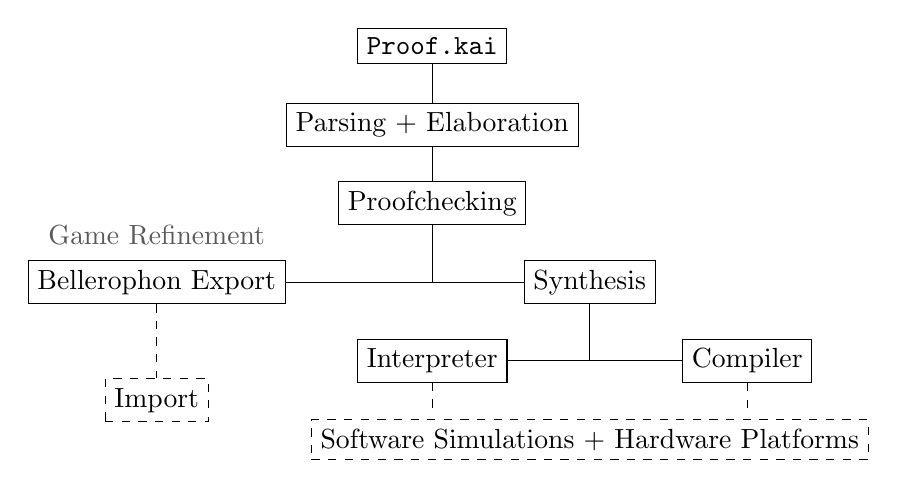
\begin{tikzpicture}
\draw (0,3) node[rectangle,draw,thin] (input) {\texttt{Proof.kai}};
\draw (0,2) node[rectangle,draw,thin] (parse) {Parsing + Elaboration};
\draw (0,1) node[rectangle,draw,thin] (pcheck) {Proofchecking};

\draw (-3.5,0.6) node (bref) {\color{vgray}Game Refinement};
\draw (-3.5,0) node[rectangle,draw,thin] (bexport) {Bellerophon Export};
\draw (-3.5,-1.5) node[rectangle,dashed,draw,thin] (bimport) {Import};

\draw (2,0) node[rectangle,draw,thin] (synth) {Synthesis};
\draw (0,-1) node[rectangle,draw,thin] (interp) {Interpreter};
\draw (4,-1) node[rectangle,draw,thin] (comp) {Compiler};

\draw (2,-2) node[rectangle,dashed,draw] (impl) {Software Simulations + Hardware Platforms};

\draw (input) -- (parse);
\draw (parse) -- (pcheck);
\draw (bexport) -- (synth);

\node[shape=coordinate] (AST) at (0,0) {};
\draw (pcheck) -- (AST);
\draw[dashed] (bexport) -- (bimport);
\draw[dashed] (comp) -- (4,-1.7);
\draw[dashed] (interp) -- (0,-1.7);

\node[shape=coordinate] (code) at (2,-1) {};
\draw (synth) -- (code);
\draw (interp) -- (code);
\draw (comp) -- (code);
  \end{tikzpicture}
\end{center}
\end{frame}
%TODO: Research Isar architecture.

\begin{frame}[t]{Arithmetic Implementation Tradeoffs}
\engineer[0.5in]~\saySad{Overflow bad!}

\begin{enumerate}
\item Scala's \texttt{spire} has computable reals.
\item Isabelle software floats: Fabian provides integration (slow).
\item Fixed-precision interval arithmetic (fast, annoying).
\end{enumerate}
\end{frame}

%\begin{frame}[t]{Code Generation}
%Control code is untrusted, so complex languages are acceptable.
%Sandbox monitor code should use simple language.
%Simple solution: Hook into VeriPhy compilation stages.
%\end{frame}

%&\begin{frame}[t]{Refinement Connects with VeriPhy}
%  \begin{itemize}
%  \item Prove game property
%  \item Synthesize controller from game proof
%  \item Automatically prove refinement
%  \item Synthesize sandbox from refined theorem and refinement proof
%  \end{itemize}
%\end{frame}

\section{Conclusion}
\begin{frame}[t]{New Work Builds on Old}
\newcommand{\cdone}{green!10}
\newcommand{\cwip}{yellow!30}
\newcommand{\cprop}{orange!30}

%\begin{figure}[tbh]
%  \centering
\begin{center}
\begin{tikzpicture}[scale=0.5]
\draw (0,3.2)  node {Logic for};
\draw (0,2.4)  node {Hybrid Systems};
\draw (0,0)   node[circle]      (CdGLcirc) {\phantom{\hspace{1.1cm}}};
\draw (0,-1) node (cdgl) {\phantom{\CdGL}};
\node[coordinate,pin={[pin distance=0.55cm,text width=2cm]320:{\S6}}] (cdgl-ref) at (cdgl) {};
\draw (0,0)   node[circle, fill=red!20,draw]      (CdGLcirc) {\phantom{\hspace{1.6cm}}};
\draw (0,-1.2) node (cdgl) {\CdGL};
\draw (0,0)   node[circle]  (dl)  {\phantom{\dL}};
\node[coordinate,pin={[pin distance=0.9cm,text width=3cm]265:{\ \ \ \ \ \ \ \ \ \S3 \S4}}] (dl-ref) at (dl) {};
\draw (dl) node[circle, fill=blue!20,draw]  {\dL};
\draw (-7, 1.3) node[rectangle,rounded corners,fill=green!20,draw,text depth=1in,text width=1.2in,text centered] (logic) {Foundations};
\draw (-7, 2.8) node[rectangle,rounded corners,fill=\cdone,draw,thin,minimum height=0.3cm] (formalization) {\dL Formalized};
\draw (-7, 1.7) node[rectangle,rounded corners,fill=\cdone,draw,thin,minimum height=0.3cm] (generalization) {\color{vgray}\dL Generalized};
\draw (-14,1.7) node {{\small\color{vgray}Not in Talk}};
\draw (-7, 0.6) node[rectangle,rounded corners,fill=\cwip,draw,thin,minimum height=0.3cm] (cgl) {Constructive \GL};
\draw (-7, -0.5) node[rectangle,rounded corners,fill=\cprop,draw,thin,minimum height=0.3cm] (cdgl) {Constructive \dGL};
\draw node[left=0.3cm of formalization] (formal-ref) {\S3.1};
\draw node[left=0.3cm of generalization] (gen-ref) {\S3.2};
\draw node[left=0.3cm of cgl] (cgl-ref) {\S5};
\draw node[left=0.3cm of cdgl] (cdgl-ref) {\S6};
\draw[dashed] (formalization) -- (formal-ref);
\draw[dashed] (generalization) -- (gen-ref);
%2.6
\draw (5, 1.4) node[rectangle,rounded corners,fill=green!20,draw,text depth=1in,text width=2.1cm,text centered] (engine) {Artifacts};
\draw (5, 2.6) node[rectangle,rounded corners,fill=\cdone,draw,thin,minimum height=0.3cm] (proofterm) {Proof Term};
\draw (5, 1.4) node[rectangle,rounded corners,fill=\cdone,draw,thin,minimum height=0.3cm] (monitors) {Monitors};
\draw (5, 0.2) node[rectangle,rounded corners,fill=\cwip,draw,thin,minimum height=0.3cm] (proofscript) {Proof Script};
\draw (5, -1) node[rectangle,rounded corners,fill=\cprop,draw,thin,minimum height=0.3cm] (controllers) {Controls};
\draw node[right=0.3cm of monitors] (monitor-ref) {\S4.1};
\draw node[right=0.3cm of controllers] (controllers-ref) {\S8};
\draw node[right=0.3cm of proofscript] (proofscript-ref) {\S7};
\draw node[right=0.3cm of proofterm] (proofterm-ref) {\S4.1};
\draw[dashed] (monitors) -- (monitor-ref);
\draw[dashed] (controllers) -- (controllers-ref);
\draw[dashed] (proofscript) -- (proofscript-ref);
\draw[dashed] (proofterm) -- (proofterm-ref);
\node[shape=coordinate] (use-anchor) at (0,-3){};
\draw (0, -5.1) node[rectangle,rounded corners,fill=green!20,draw,text depth=1.6cm,text width=2.1in,text centered] (luser) {Usability};
\draw (0.3, -4.7) node[rectangle,rounded corners,fill=\cprop,draw,thin,minimum height=0.3cm] (monitors)    {Simplicity};
\draw (0.1, -4.7) node[rectangle,rounded corners,fill=\cprop,draw,thin,minimum height=0.3cm,text width=4.8cm] (lop)    {Lines of Model/Proof};
\draw (-2.9, -6.05) node[rectangle,rounded corners,fill=\cprop,draw,thin,minimum height=0.3cm,text width=2cm] (modelmistake) {Model Bugs};
\draw (2.4, -6) node[rectangle,rounded corners,fill=\cprop,draw,thin,minimum height=0.3cm,text width=2.4cm] (maintainable) {Maintainable?};
\draw node[right=0.3cm of maintainable] (maintain-ref) {\S7};
\draw node[right=0.3cm of lop] (lop-ref) {\S7};
\draw[->,very thick] (logic) -- (CdGLcirc);
\draw[->,very thick] (CdGLcirc) -- (engine);
\draw[dashed] (CdGLcirc) -- (luser);
\draw[dashed] (lop) -- (lop-ref);
\draw[dashed] (maintainable) -- (maintain-ref);
\end{tikzpicture}
\end{center}
\end{frame}


%TODO: Possibly subdivide for kaisar theory work.
\begin{frame}[t]{Thesis is Big, but Doable}
% Upcoming deadlines:
%  CAV Jan 2020
%  IJCAR Feb 2020
%  FM Mar 2020
%  RV May 2020
Timeline: $\approx$\textbf{14 months}, optimistic
\begin{itemize}
\item 1 month (Nov) \CGL theory
\item 1 month (Dec) Game refinements
\item 1 month (Jan) Revisions and resubmissions
\item 1 month (Feb) Kaisar theory
\item 2 months (Mar-Apr) Kaisar proofchecking implementation
\item 2 months (May-Jun) Kaisar \ProofPlex monitoring implementation
\item 1 month (Jul) Generalize ground robotics case study to \CdGL
\item 2 month (Aug-Sep) Further revisions and resubmissions
\item 3 months (Oct-Dec) Write thesis document, defend\pause
%\item 1 month Productivity lost due to insanity
\end{itemize}
Amenable to change (i.e., not on job market this year)
\end{frame}

%TODO: Plans are important but it's hard to discuss without context
\begin{frame}[t,allowframebreaks]{Backup Plans are in Place}
\textbf{CdGL Backup Plans:}
\begin{itemize}
\item If $\ddiamond{\text{ODE}}{}$ rules are infeasible, pursue simplified ``solve'' axiom
\item If arbitrary computable terms are infeasible, use polynomial terms with limited use of semialgebraic witnesses
\item If model-predictive control is infeasible, focus on synthesizing assignments and conditionals
\item If refinement work fails, can directly reimplement sandboxing on games or rely on manual refinement
\end{itemize}
\framebreak
\textbf{Kaisar Backup Plans:}
\begin{itemize}
\item If usability results are weak, extend theory results
\item If nominal features do not provide desired benefits, refocus efforts on modularity
\item If implementation tasks become infeasibly large, pursue tighter integration with \KeYmaeraX code base or cut ``Export to Bellerophon proof'' feature
\end{itemize}
\framebreak

{\textbf{Robot Backup Plans:}
\begin{itemize}
\item Generalize robot model to improve synthesized monitor
\item Minimize proof complexity to support easy synthesis
\item Pursue a mix of hardware and simulation evaluations based on needs:
\item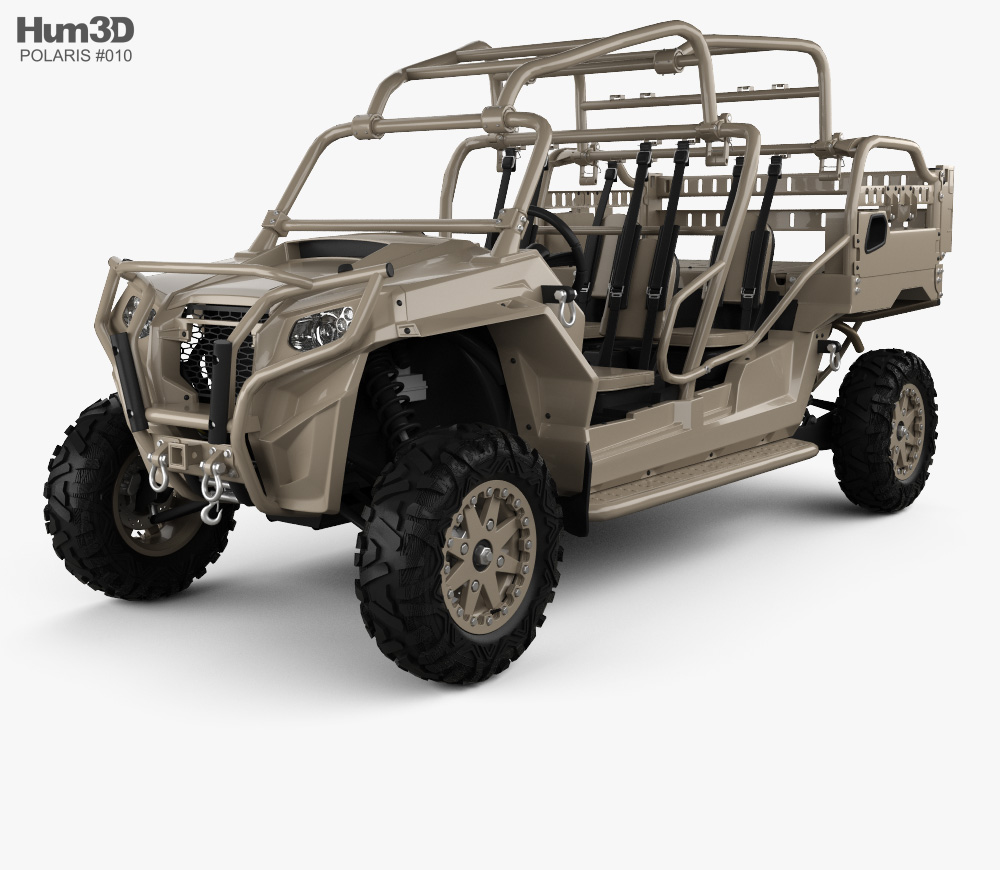
\includegraphics[width=1.2in]{img/mrzr.jpg}\\
Polaris MRZR (access on limited dates only)
\item 1-10th scale RC Car (full access)
\item AirSim simulator
\end{itemize}}
\end{frame}


\begin{frame}[t]{Thesis Makes the Whole Crew Happy}
  \begin{tabular}{lll}
    \ah{1}{\engineer} & \ah{1}{\logician} & \ah{1}{\logicuser}\\
    \acl{1}{\sayHappy{Full synthesis suite!}} & \acl{1}{\sayHappy{Formal foundations!}} & \acl{1}{\sayHappy{Structured proofs!}}
  \end{tabular}
\end{frame}

% \newcommand{\ctrlspike}{\Large{\bf C\dag}}
% \newcommand{\ctrlfault}{\Large{\bf C\Lightning}}
% \newcommand{\plantfault}{\Large{\bf P\Lightning}}
% \newcommand{\ctrlrestore}{\Large{\bf C\tiny\Checkmark}}
% \newcommand{\graphscale}{0.4}
% \newcommand{\obsforward}{\Large{\bf{Ob{+}}}}
% \newcommand{\obsback}{\Large{\bf{Ob{-}}}}
% \newcommand{\obshalt}{\Large{\bf{Ob{0}}}}
% \newcommand{\graphwidth}{6.5in}
% \newcommand{\graphheight}{8.5cm}
% %TODO: Do we need two evaluation slides?
% \begin{frame}[t]{Code Executed on GoPiGo Robot}
% \begin{textblock}{8}(1.9,2.7)
% Operational Suitability? \\
% Arithmetic Precision?
% \end{textblock}
% \begin{textblock}{8}(12,2)
% 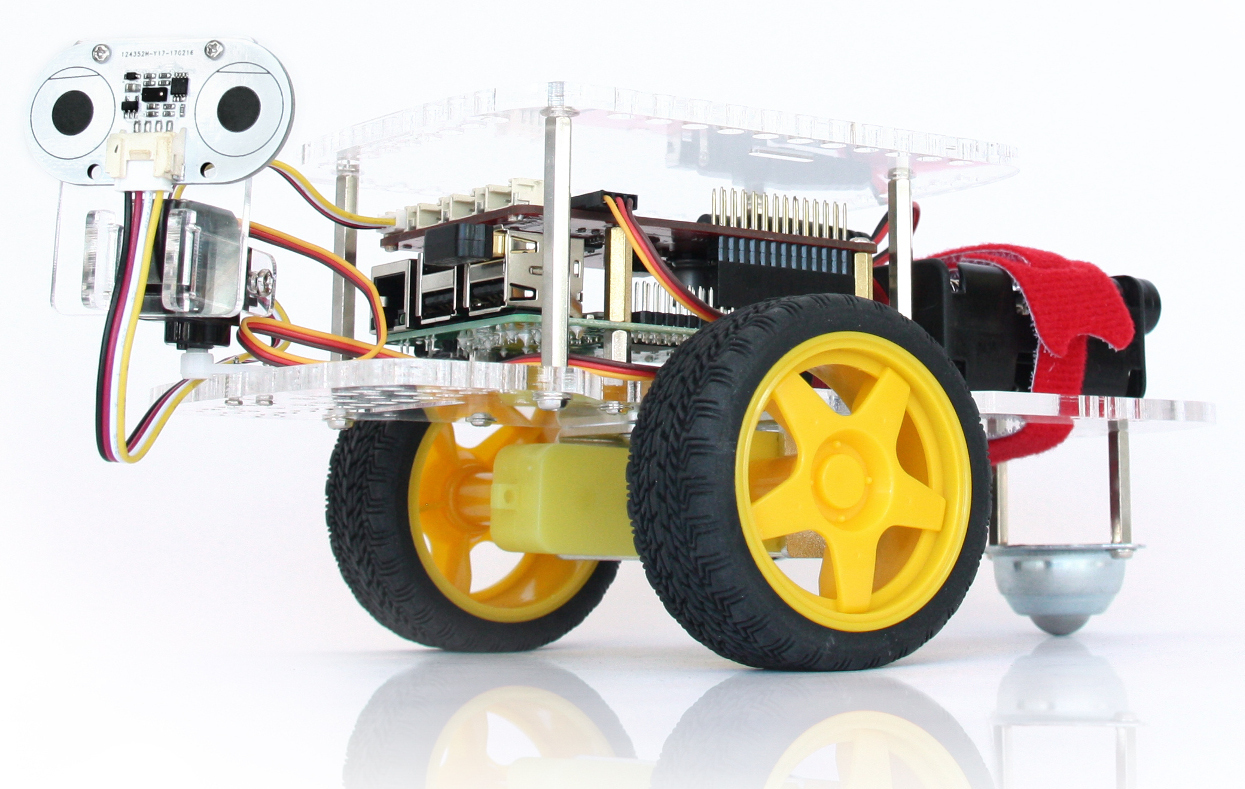
\includegraphics[width=1.2in]{img/gopigo3.jpg}\\
% \end{textblock}
% \begin{textblock}{100}(1,5.2)
%     \begin{tabular}{lr}
% \begin{tikzpicture}[trim axis left,scale=\graphscale]
%       \begin{axis}[ scale only axis, width=\graphwidth, height=\graphheight,
%         ytick scale label code/.code={}, xtick scale label
%         code/.code={}, scaled x ticks=base 10:-3, scaled y ticks=base
%         10:-4, x label style={at={(axis description
%             cs:1.03,0)},anchor=north east}, xlabel={time
%           $[\textit{s}]$}, y label style={at={(axis description
%             cs:0,1.0)},rotate=-90,anchor=south west},
%         ylabel={distance $[\textit{cm}]$}, grid=both, axis on top,
%         cycle list name=auto, clip=false, enlargelimits=false, legend style={at={(0.95,0.95)}}]
%         \addplot+[myblue,mark=,solid,ultra thick]
%         table[x=time,y=d,skip first n=1,col sep=comma]
%         {correct100.csv};
%         \addlegendentry{Controller A (correct)};
%         \coordinate (fault1) at (axis cs:4400,46000);
%         \addplot+[vgreen,mark=,ultra thick] table[x=time,y=d,skip
%         first n=1,col sep=comma]
%         {ctrlbug100.csv};
%         \addlegendentry{Controller B (faulty)};
%         \node[coordinate,pin={[align=center,pin
%           distance=0.5cm]90:{\textcolor{vgreen}{\ctrlspike}}}] at
%         (axis cs:2700,460000) {};
%         \addplot+[myyellow,mark=,dashed,ultra thick]
%         table[x=time,y=d,skip first n=1,col sep=comma]
%         {backwards100.csv};
%         \addlegendentry{Malicious obstacle};
%         \coordinate (fault2) at (axis cs:3300,24000) {};
%         \node[coordinate,pin={[align=center,pin
%           distance=0cm]180:{\textcolor{myyellow}{\ctrlspike}}}] at
%         (axis cs:1900,450000) {}; \node[coordinate,pin={[pin
%           distance=0cm]260:{\textcolor{myyellow}{\plantfault}}}] at
%         (axis cs:3740,2000) {};
%         % BB%\node[coordinate,pin=below left:{\plant violation}] at (axis cs:3740,2000) {};
%         \addplot+[black,mark=,ultra thick] table[x=time,y=d,skip first
%         n=1,col sep=comma]
%         {actoffsetSafe100.csv};
%         \addlegendentry{Small disturbance};
%         % \node[coordinate,pin={[align=center,pin
%         % distance=1cm]60:{\Lightning~Fault becomes\\
%         % safety-critical,\\ fallback engaged}}] at (axis
%         % cs:5060,19600) {};
%         \coordinate (fault3) at (axis cs:5060,19600) {};
%         \node[coordinate,pin={[align=center,pin
%           distance=0cm]70:{\textcolor{black}{\ctrlspike}}}] at (axis
%         cs:2860,492600) {}; %(axis cs:2640,486000) {};
%         \node[coordinate,pin={[align=center,pin
%           distance=0.2cm]120:{\ctrlrestore}}] at (axis cs:8800,57000)
%         {}; \node[coordinate,pin={[align=center,pin
%           distance=0.2cm]205:{\ctrlfault}}] at (axis cs:9020,4200) {};
%         % Fault again\\ safety-critical,\\
%         % \coordinate (fault4) at (axis cs:9020,4200) {};
%         \addplot+[myblue,mark=,dashed,ultra thick]
%         table[x=time,y=d,skip first n=1,col sep=comma]
%         {actoffsetUnsafe100.csv};
%         \addlegendentry{Large disturbance};
%         \node[coordinate,pin={[align=center,pin
%           distance=0cm]180:{\textcolor{myblue}{\ctrlspike}}}] at (axis
%         cs:2600,450000) {}; \node[coordinate,pin={[align=center,pin
%           distance=0cm]160:{\textcolor{myblue}{\ctrlfault}}}] at (axis
%         cs:4200,3000) {};
%         \node[coordinate,pin={[align=center,pin
%           distance=0cm]270:{\textcolor{myblue}{\plantfault}}}] at
%         (axis cs:6600,2000) {};
%         \node[coordinate,pin={[align=center,pin distance=0.2cm]20:{\textcolor{vgreen}{\ctrlfault}}}] at (fault1) {};
%         \node[coordinate,pin={[align=center,pin
%           distance=0cm]180:{\textcolor{myyellow}{\ctrlfault}}}] at
%         (fault2) {}; \node[coordinate,pin={[align=center,pin
%           distance=0cm]240:{\textcolor{black}{\ctrlfault}}}] at
%         (fault3) {};
%       \end{axis}
%     \end{tikzpicture}
% &\vspace{-0.8cm}
% \begin{tikzpicture}[trim axis left,scale=\graphscale]
% \begin{axis}[
% scale only axis,
% width=\graphwidth,
% height=\graphheight,
% ytick scale label code/.code={},
% xtick scale label code/.code={},
% scaled x ticks=base 10:-3,
% scaled y ticks=base 10:-4,
% x label style={at={(axis description cs:1.03,0)},anchor=north east},
% xlabel={time $[\textit{s}]$},
% y label style={at={(axis description cs:0,1)},rotate=-90,anchor=south west},
% ylabel={distance $[\textit{cm}]$},
% grid=both,
% axis on top,
% cycle list name=auto,
% clip=false,
% enlargelimits=false,
% legend style={at={(0.95,0.95)}}
% ]
%  \addplot+[myblue,mark=,ultra thick] table[x=time,y=d,skip first n=0,col sep=comma] {sim/correct100.csv};
% \addlegendentry{Controller A (correct)};
%  \addplot+[vgreen,mark=,ultra thick] table[x=time,y=d,skip first n=0,col sep=comma] {sim/ctrlbug100.csv};
% \addlegendentry{Controller B (faulty)};
% \node[coordinate,pin={[align=center,pin distance=0.1cm]70:{\textcolor{vgreen}{\ctrlspike}}}] at (axis cs:2445,460000) {};
% % Fault becomes\\ safety-critical,\\ f
% \node[coordinate,pin={[align=center,pin distance=-0.1cm]45:{\textcolor{vgreen}{\ctrlfault}}}] at (axis cs:4109,46000) {};
%  \addplot+[myyellow,mark=,ultra thick] table[x=time,y=d,skip first n=0,col sep=comma] {sim/backwards100.csv};
% \addlegendentry{Approaching obstacle};
% \node[coordinate,pin={[align=center,pin distance=0.2cm]265:{\textcolor{myyellow}{\obsforward}}}] at (axis cs:2074,422000) {};
% \node[coordinate,pin={[align=center,pin distance=0cm]-70:{\textcolor{myyellow}{\obsback}}}] at (axis cs:4295,18000) {};
% \node[coordinate,pin={[align=center,pin distance=0cm]-0:{\textcolor{myyellow}{\obshalt}}}] at (axis cs:5774,486000) {};
% \addplot+[black,mark=,ultra thick] table[x=time,y=d,skip first n=0,col sep=comma] {sim/forwardObstCompensatesUnsafeActoffset100.csv};
% \addlegendentry{Robot follows obstacle};
% \node[coordinate,pin={[align=center,pin distance=0.2cm]86:{\obsforward}}] at (axis cs:5218,214000) {};
% \end{axis}
% \end{tikzpicture}
%     \end{tabular}
% \end{textblock}
%\renewcommand{\ctrlspike}{\small{\bf C\dag}}
%\renewcommand{\ctrlfault}{\small{\bf C\Lightning}}
%\renewcommand{\plantfault}{\small{\bf P\Lightning}}
%\renewcommand{\ctrlrestore}{\small{\bf C\tiny\Checkmark}}
%\renewcommand{\obsforward}{\small{\bf{Ob{+}}}}
%\renewcommand{\obsback}{\small{\bf{Ob{-}}}}
%\renewcommand{\obshalt}{\small{\bf{Ob{0}}}}

%\begin{textblock}{100}(3,12.5)
%Control Fault \ctrlfault{}, Plant Fault \plantfault{}, Control Spike \ctrlspike{}, Obstacle Motion {\textbf{Ob}}
%\end{textblock}
%\end{frame}

% https://github.com/jsford/FFAST

\appendix
\section{Appendix}

%TIMED: 1:27:00,  87 mins, needs to be 45, cut 42 mins, ~50%
\begin{frame}[t,allowframebreaks]{TODO List}
  \begin{itemize}
%  \item Identify nonsense slides, e.g., where background info, connecting info, explanation, context are needed.
%  \item Try to fix nonsense by Wednesday meeting.
%  \item In meeting, discuss: Slides, resubmission plans, whether to do extra practice talks
  \item Research related works which inform design questions, e.g., Isar architecture and software engineering works
  \item Identify questions likely to be asked by committee, prepare answers
  \item Identify additional figures that improve slides, make said figures
  \item General polish
  \item Practice talk in lab meeting, Oct 22
  \item Test Skype connection with Tobias
  \item Keep document updated with insights and plans arising from the talk editing, and publishing status
  \item Explore ML programs as realizers
  \end{itemize}
\end{frame}

\section<presentation>*{\appendixname}
\subsection<presentation>*{For Further Reading}

\begin{frame}[t, allowframebreaks]
\frametitle{References}
\bibliographystyle{amsalpha}
\bibliography{proposal,platzer,verified-pipeline,hilbert-epsilons,ground-robotics,verified-dL,constructive-games,kaisar}
\end{frame}

\end{document}